\documentclass[11pt,a4paper]{article}

\usepackage [english]{babel}
\usepackage [utf8]{inputenc}
%\usepackage[latin1]{inputenc}para utilizar acentos pero aqui no funciona (en otros si)
\usepackage [T1]{fontenc}
\usepackage{graphicx}
\usepackage{graphics}
\graphicspath{ {Figuras/} } %Para buscar las imágenes en otra carpeta
\usepackage{amsfonts} %Para poder escribir letras como la matriz identidad
\usepackage{mathrsfs} %Para poder escribir letras como la H del el espacio de Hilbert
\usepackage{slashed} % para la d barra cruzada
\usepackage{amsmath}
\usepackage{amssymb}
\usepackage{makeidx}
\usepackage{hepunits} %para poder utilizar unidades
\usepackage[version=3]{mhchem} %para poder escribir los simpolos atómicos y químicos
%\usepackage{hep}
\usepackage[left=2.5cm,right=2.5cm,top=2.5cm,bottom=2.5cm]{geometry}
%\renewcommand{\figurename}{ Figura}
%\usepackage[labelsep=endash]{caption}

%\usepackage[figurename=\bold{Figura}]{caption}
%\usepackage [labelformat=empty]{caption}
%\usepackage{wrapfig} %for I can use wrapfigure
\usepackage[font={small, up}]{caption}
\usepackage{subfigure}
\usepackage{hyperref} %hipervinculos del índice
\setlength{\parindent}{4em} %para que interprete la linea en blanco como un \parragraph{}
\setlength{\parskip}{1em}
%\usepackage{subcaption}

\renewcommand{\baselinestretch}{1.15}
%\renewcommand{\thefigure}{}

%para aumentar el espacio entre elementos del índice
\usepackage{setspace}

\bibliographystyle{unsrthep}



\begin{document}
\captionsetup[figure]{labelfont={bf},labelformat={default},labelsep= endash,name={Figura}}
\begin{titlepage}

\begin{center}
\vspace*{-1in}
\vspace*{1 cm}
\begin{figure}[htb]
\begin{center}

\includegraphics[scale=1]{Logo1.png}
\end{center}
\end{figure}
\vspace*{2 cm}


{\huge TRITIUM project}\\
\vspace*{0.2in}
\vspace*{0.6in}
\end{center}
\vspace*{-1in}
\begin{center}
\vspace*{0.25 cm}


\begin{figure}[htb]
\begin{center}

\includegraphics[scale=0.1]{Logo2.jpg} 
\end{center}
\end{figure}
\vspace*{1 cm}

\begin{large}
\textbf{{\large Internal report}}\\
\rule{80mm}{0.1mm}\\
%\vspace*{2 cm}

\end{large}
\vspace*{0.2in}
\begin{Large}
\textbf{\LARGE Design, construction and results of tritium laboratory prototypes of Tritium detector} \\
\end{Large}
%\vspace*{0.3in}
\vspace*{1 cm}

\begin{large}
Marcos Martínez Roig\\
\today
\end{large}
\end{center}

%\vspace*{0.3in}
%\rule{80mm}{0.1mm}\\
%\vspace*{0.1in}
\begin{large}
\begin{flushright}
\item[\bf Supervisors:\hspace{4cm} ]\quad  \\ José Díaz Medina\\
Nadia Yahlali Haddou\\
\end{flushright}
\end{large}

\end{titlepage}



%\newpage
\tableofcontents
\newpage

%%%%%%%%%%%%%%%%%%%%%%%%%%%%%%% MAIN BODY %%%%%%%%%%%%%%%

\section{Introduction}  \label{sec:Introduction}
The laboratory prototypes, which have been developed by Valencia research group in the framework of Tritium project, are detailed in this report. 

The Tritium detector are focused on monitoring of low radiactive tritium activities in water which is released for nuclear power plants. It is based on the deteccion of tritium radiation by scintillator fibers which will be read out by several photosensors (PMTs or SiPM arrays).

The fibers, which have been used in all prototypes, were buying in Saint-Gobain company, model BCF-12, whose diameter is $1~\mm$. In all the cases these fibers were cutted and polished at a distance of $20~\cm$. 

For the cutting process, the device, which is shown in the figure \ref{fig:Cuttingdevice}, was developed and built in the IFIC and the results was checked to the microscope.

\begin{figure}[htb]
\centering
{
%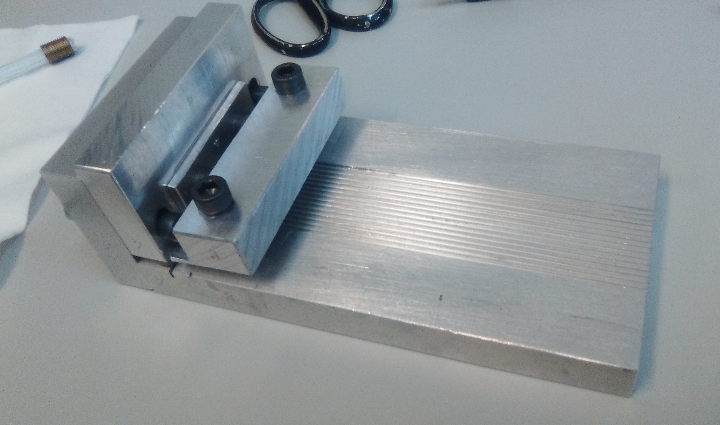
\includegraphics[scale=0.25]{Guillotina1.png} 
}
\caption{Cutting device \label{fig:Cuttingdevice}}
\end{figure} 

For the polishing process, the machine, which is shown in figure \ref{fig:PolishingMachine}, was developed and built at IFIC. This machine is controlled with arduino technology and it reproduces and automates the manual method recommended by Saint-Gobain. 

\begin{figure}[htb]
\centering
{
%\includegraphics[scale=0.25]{PolishingMachine.png} 
}
\caption{Polishing machine \label{fig:PolishingMachine}}
\end{figure} 

The results of this polishing process were verified under a microscope (figure \ref{fig:VisualResultPolish}) and with measurements of the light collection (figure \ref{fig:ResultPolish}). 

\begin{figure}[htbp]
\centering
\subfigure[Final face of the fiber before the polishing process \label{fig:VisualBeforePolish}]{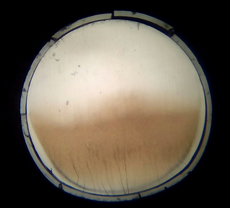
\includegraphics[width=60mm]{./Figuras/NoPolished.png}}\hspace{10mm}
\subfigure[Final face of the fiber after the polishing process \label{fig:VisualAfterPolish}]{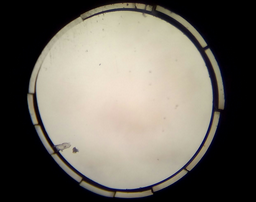
\includegraphics[width=70mm]{./Figuras/Polished.png}}
\caption{Visual result of the polishing process under the microscope} \label{fig:VisualResultPolish}
\end{figure}

\begin{figure}[htbp]
\centering
\subfigure[Measurement of the light produced in a bunch of $25$ fibers of $20~\cm$ due to the \ce{^{90}Sr} source \label{fig:SrPolish}]{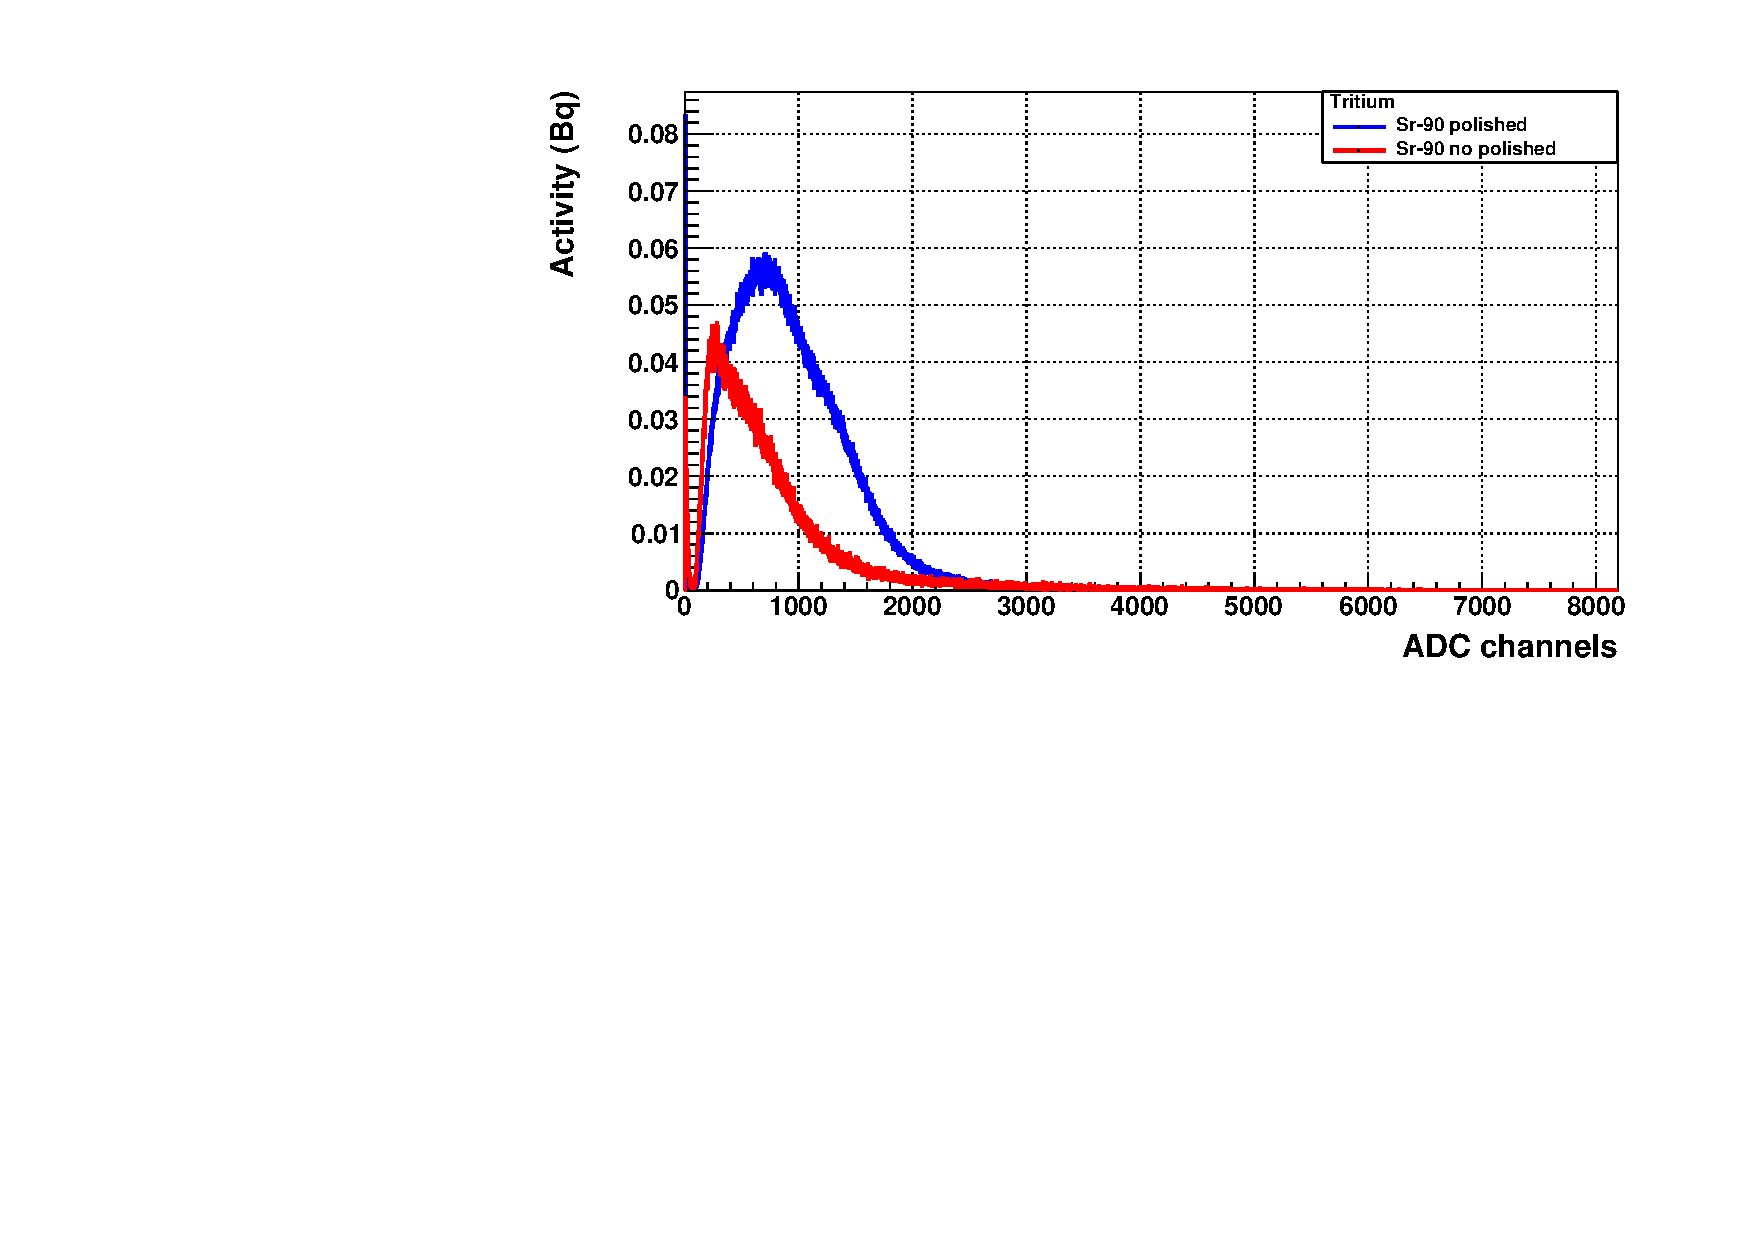
\includegraphics[width=77mm]{./Figuras/Sr_90.pdf}}
\subfigure[Measurement of the light produced in a bunch of $25$ fibers of $20~\cm$ due to the \ce{^{60}Co} source \label{fig:CoPolish}]{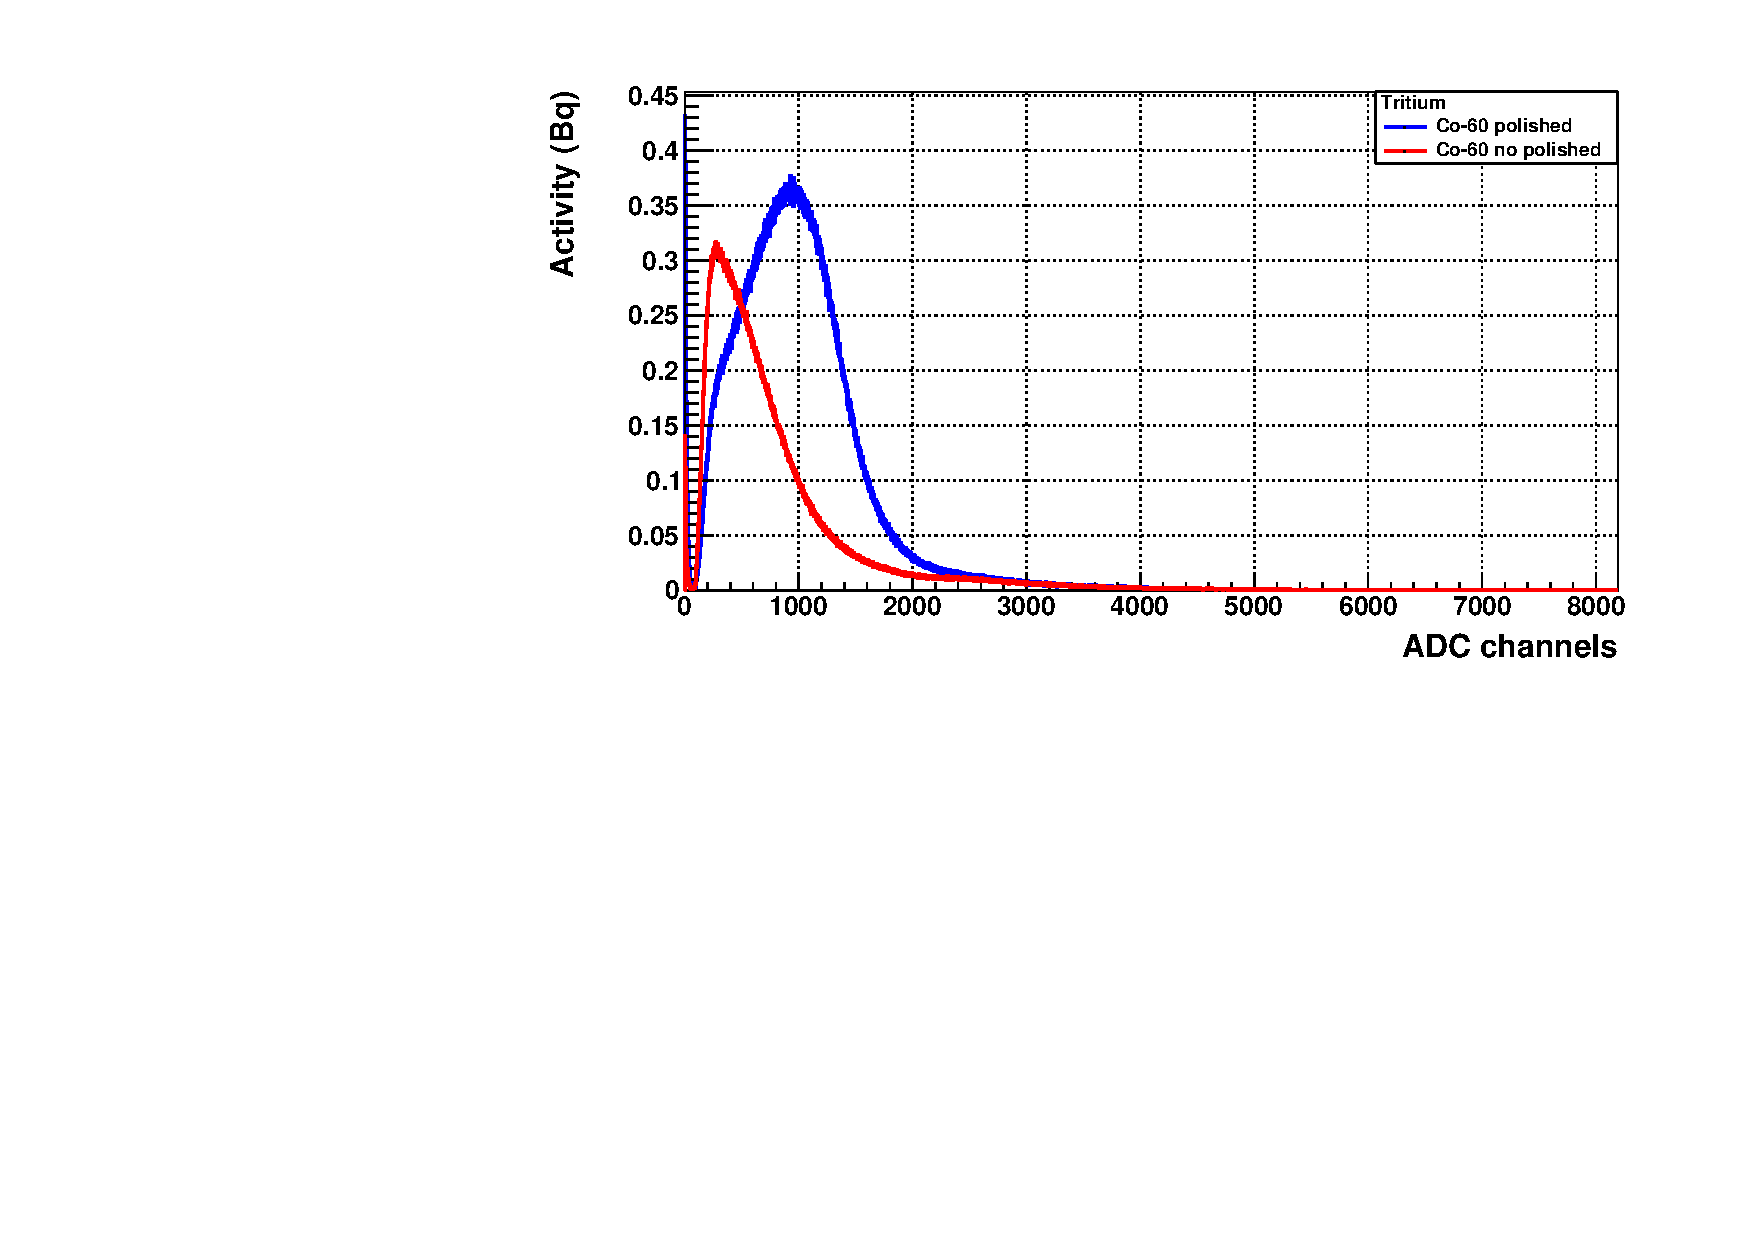
\includegraphics[width=77mm]{./Figuras/Co_60.pdf}}
\caption{Cuantification of the improvement of polishing process} \label{fig:ResultPolish}
\end{figure}

From this measurements the improvement in the light collection was quantified in around $50\%$ for $\beta$ radiation, as you can see in the table \ref{TablePolish}

\begin{table}
\centering
\begin{tabular}{l | c | c | c | c}
Source & Not polished & Polished & Improvement\\
\hline \hline
Sr-90 & 33 & 64  & 48.44 \% \\ 
Co-60 & 243 & 424 & 74.49 \% 
\end{tabular}
\caption{Counts/second due to each source \label{TablePolish}}
\end{table}

We have to take into account that in the final detector the water will flow through the detector, but it is not necessary for laboratory tests. The laboratory prototypes will be water hermetic to reduce the difficulty of these prototypes since the security requirements are strong due to the high activities contained in them.

The different prototypes, which have been created in Valencia, were filled following the same protocol which was developed in the IFIC. This protocol is explained in the seccion \ref{sec:FillInPrototypes}. All measurements were made inside a special black box which is light tight

In this work we will discuss the problems that was found in each prototype and how the next version overcomed these problems. On top of that, we will speak about the improvements that was included in each prototype and how it affect to our detector.

%\newpage
\section{Tritium-IFIC 0 prototype} \label{sec:TritiumIFIC0}
The name of the fist prototype, which was developed in Valencia, is Tritium-IFIC 0 and it was the proof where we could check that we were able to detect tritium in water samples with this technology. This protoype is shown in the figure \ref{fig:Tritium_IFIC_0}.

\begin{figure}[htb]
\centering
{
%\subfloat[Front view]{
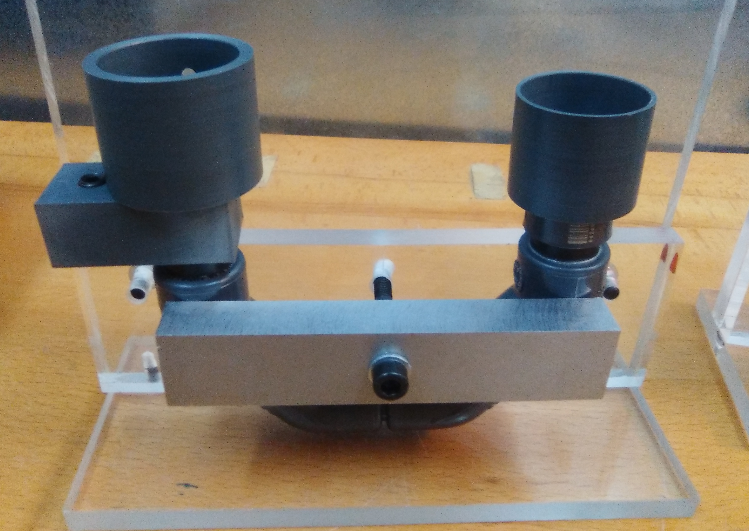
\includegraphics[scale=0.25]{Prototipodelantetapon.png} 
}
{
%\subfloat[Back view]{
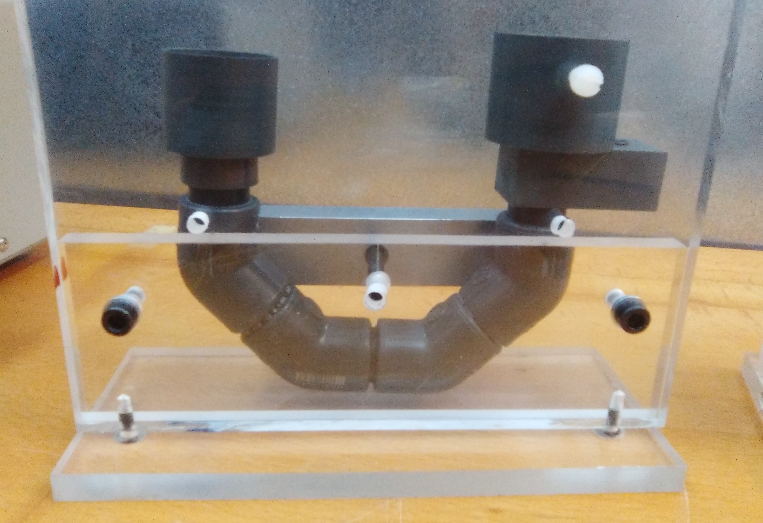
\includegraphics[scale=0.25]{PrototipoDetrastapon.png} 
}
\caption{Tritium-IFIC 0 prototype. Front view (left) and back view (right) \label{fig:Tritium_IFIC_0}}
\end{figure} 

This prototype contains $35$ scintillating fibers read out by two PMTs in coincidence, which was bought from Hamamatsu company, model R8520. 

These fibers were contained in a PVC vessel because it is a safe material widely used in plumbing. On top of that, as you can see in the figure \ref{fig:Tritium_IFIC_0}, it has a U-shape because it is safer. 

Two identical prototypes were built with internal diameter of $15~\mm $ and an internal volume of $39~\cm^2$, which was verified with various fill tests. The first prototype, which was used for getting the tritium signal of the system, was filled with tritium solution with high activity ($53.385~\mega\becquerel/\liter$) and the other prototype, which was used for getting the background signal of the system, was filled with hiper-pure water. 

These prototypes is hold with a methalic and steel structure, which was constructed in the IFIC workshop. The electronic circuit used for processing the signals of each circuit was the same and its electronic scheme is shown in the figure \ref{fig:Electronic_scheme}.

\begin{figure}[htb]
\centering
{
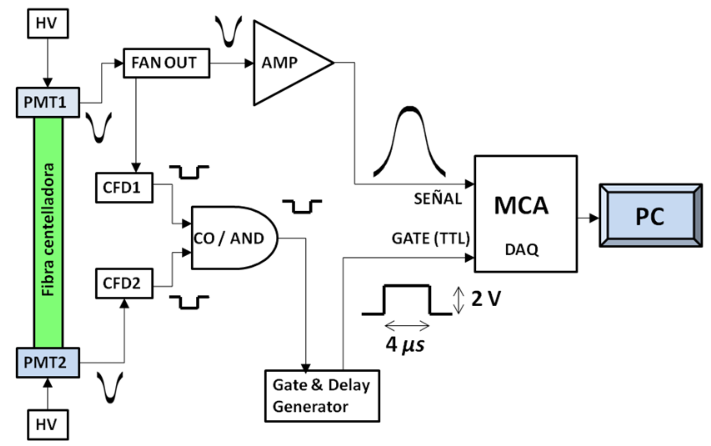
\includegraphics[scale=0.4]{Esquemaelectronico.png} 
}
\caption{Electronic scheme used for analysing the signal of Tritium-IFIC 0 prototype \label{fig:Electronic_scheme}}
\end{figure} 

It is based on several NIM technology modules with which we amplify the signal of the detector and make coincidence between both PMTs in order to remove the electronic noise of the PMTs. 

The measurement obtained from both prototypes are shown in the figure \ref{fig:SignalsTritiumIFIC0} and the difference between both signals, which correspond to the tritium signal, are shown in the \ref{fig:ClearSignalTritiumIFIC0}. 

\begin{figure}[htbp]
\centering
\subfigure[Signal and Background of Tritium-IFIC 0 \label{fig:SignalsTritiumIFIC0}]{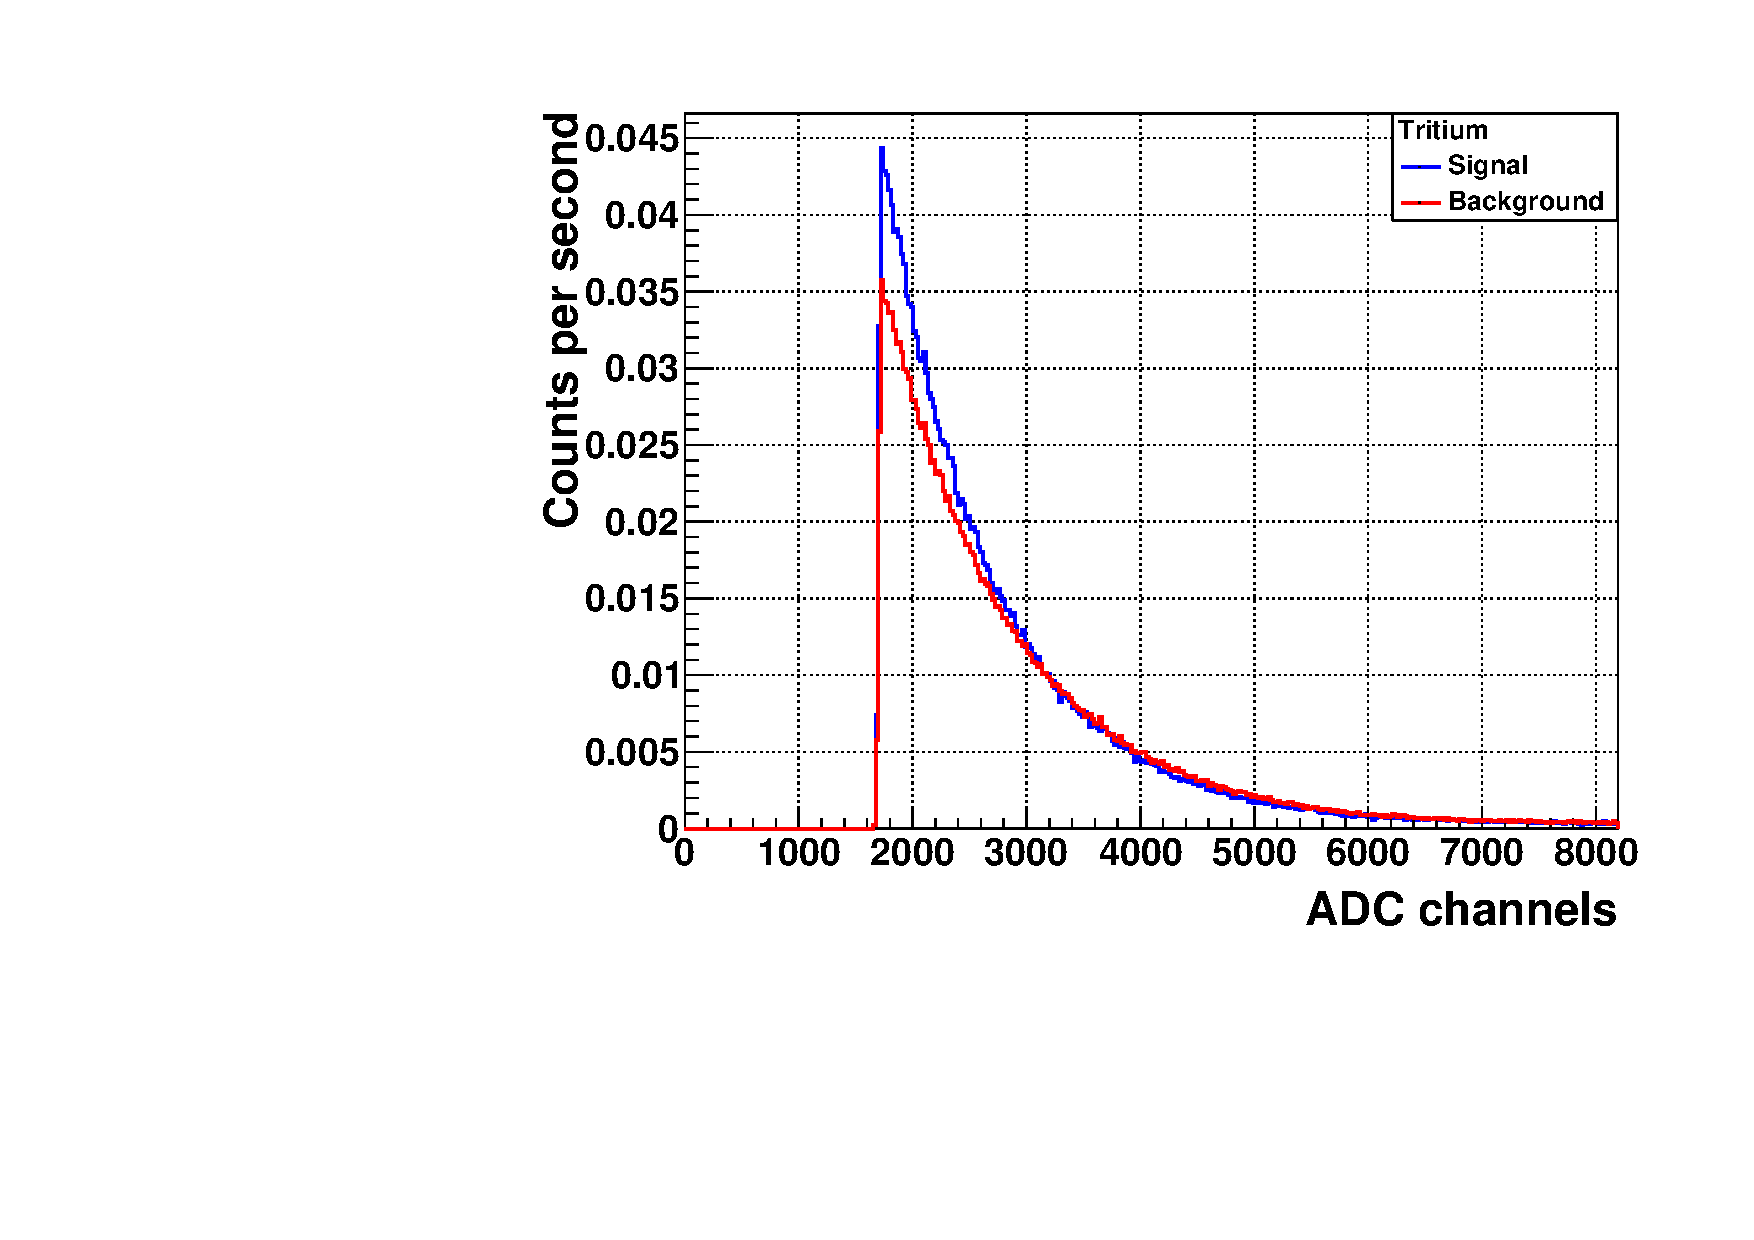
\includegraphics[width=77mm]{./Figuras/tritio-fondo_Tritium0.pdf}}
\subfigure[Clear signal of tritium \label{fig:ClearSignalTritiumIFIC0}]{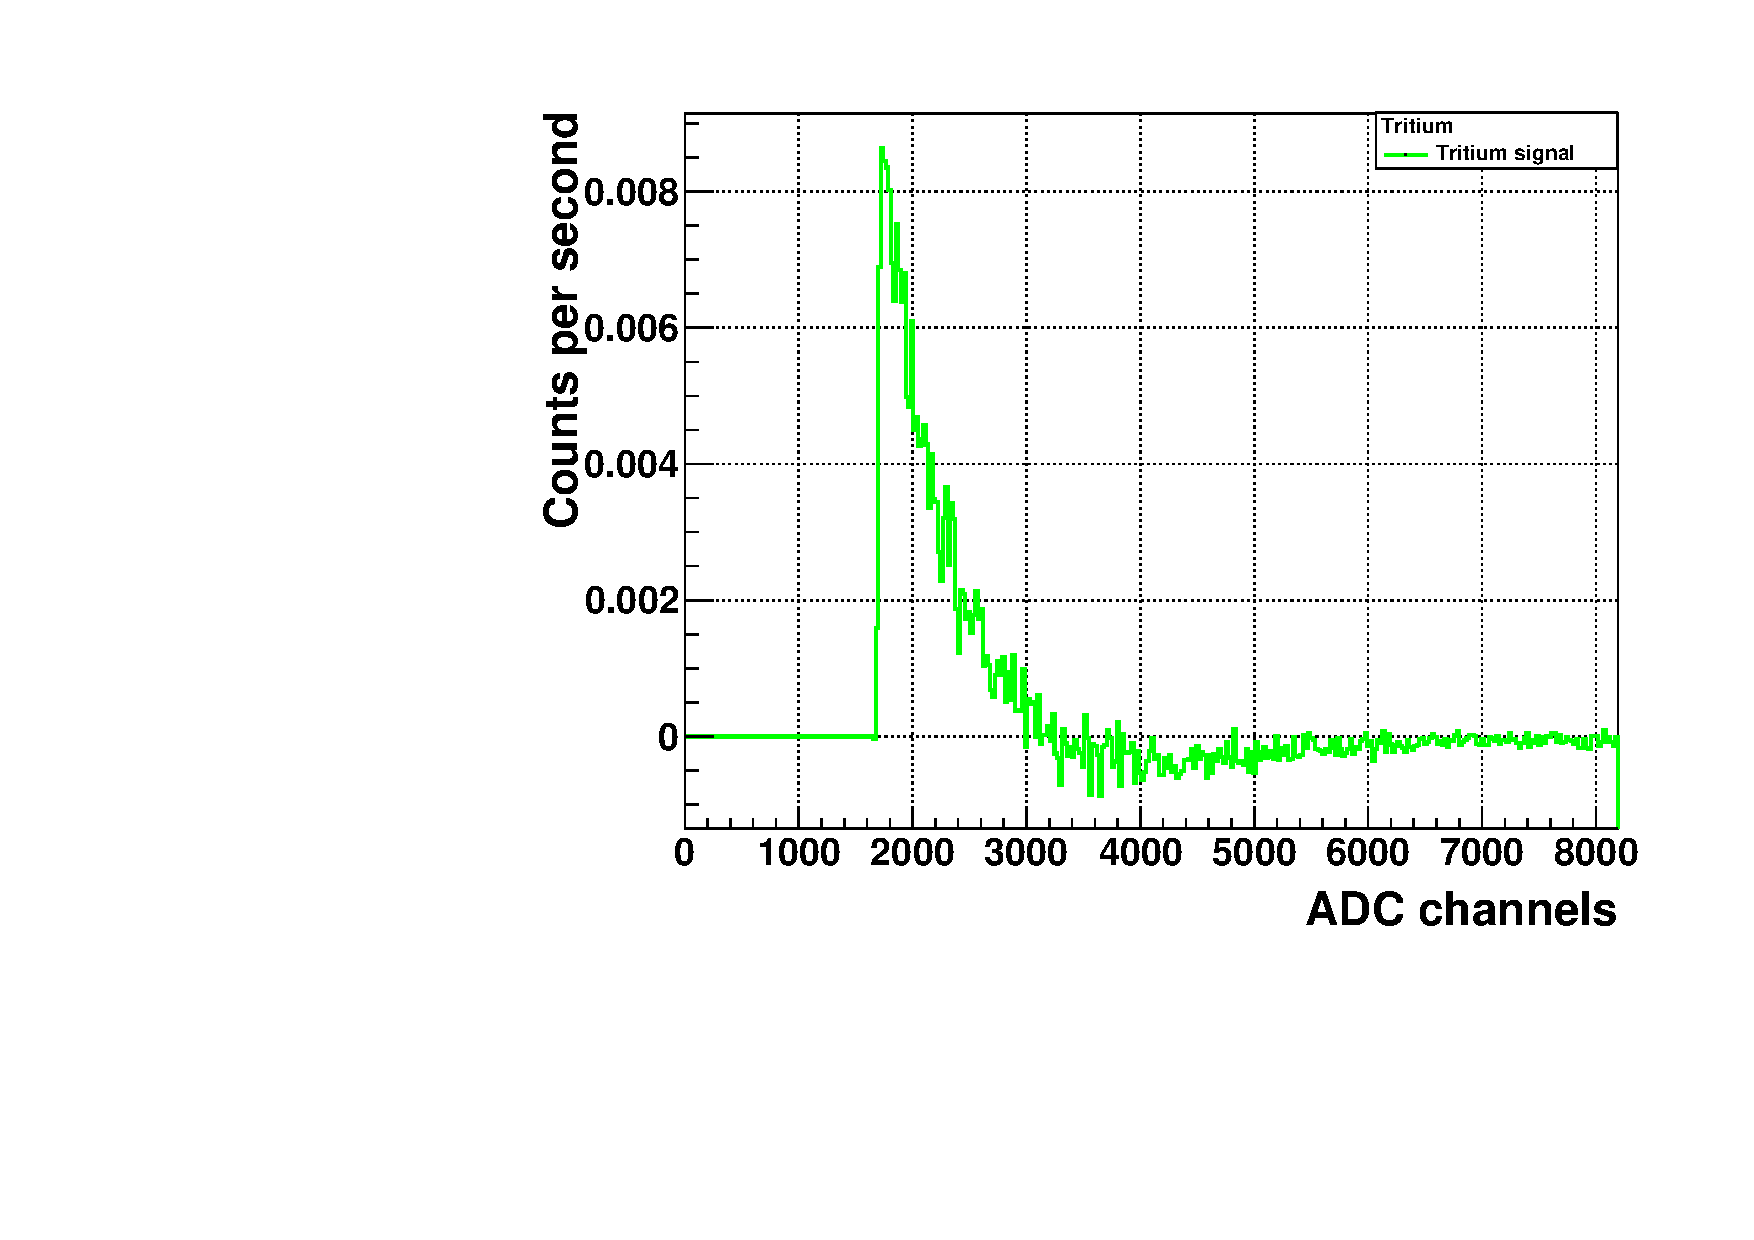
\includegraphics[width=77mm]{./Figuras/tritiumsignal_Tritium0.pdf}}
\caption{Signals of Tritium-IFIC 0 prototype.} \label{fig:Tritium_IFIC_0_Signals}
\end{figure}

In this experience we have obtained $0.199$ counts per second for this activity, which means that the effiecincy of our detector is $ \varepsilon_{det} = 3.728 \cdot 10^{-6}~(\ce{counts}/\sec)/(\kilo\becquerel/\liter)$. We know that the efficiency of this type of detectors scales with the active surface so we can obtain the specific efficiency. It is the efficiency normalized to the active surface of our detector ($A_{suf} = 219.8~\cm^2$) whose value is $ \varepsilon_{esp} = \varepsilon_{det}/A_{suf} =  1.695 \cdot 10^{-8}~(\ce{counts}/\sec)/(\cm^2\kilo\becquerel/\liter)$. 

This value of specific efficiency is two orders smaller than the one get with other similar detectors (reference of the thesis) so we looked for the reason of this fact. 

We viewed the surface of the scintillator fibers under the electron microscope and, as you can see in the figure \ref{fig:FiberSurfaceElectronMicroscope}, we found that this surface was not as good as we though. 

\begin{figure}[htbp]
\centering
%\subfigure[]
{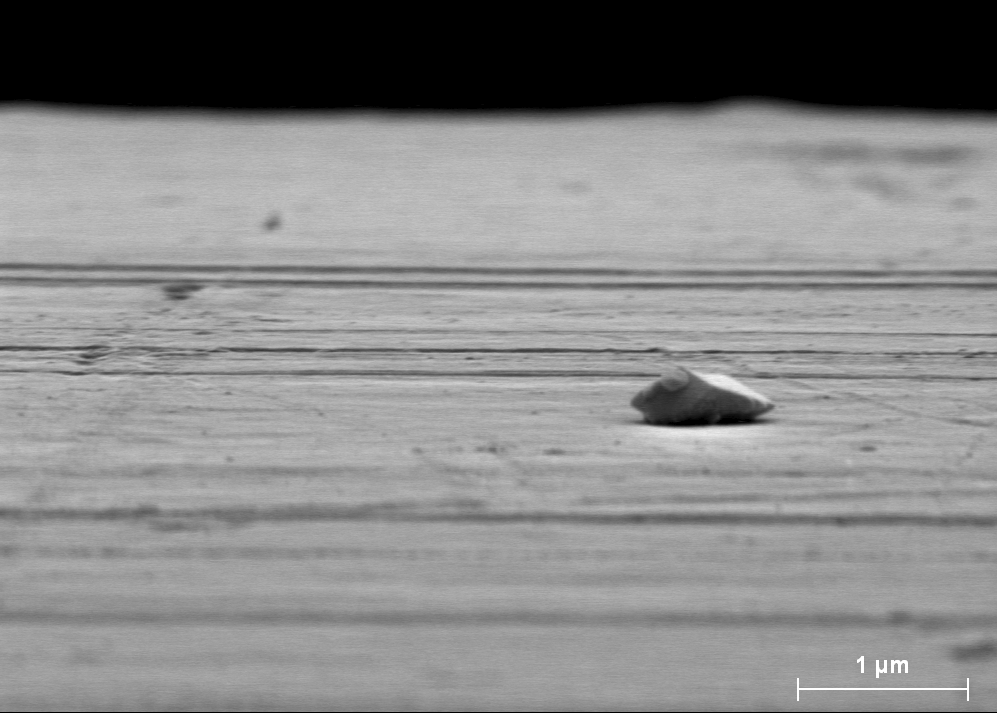
\includegraphics[width=70mm]{./Figuras/sinclad_3_SE.png}}\hspace{10mm}
%\subfigure[]
{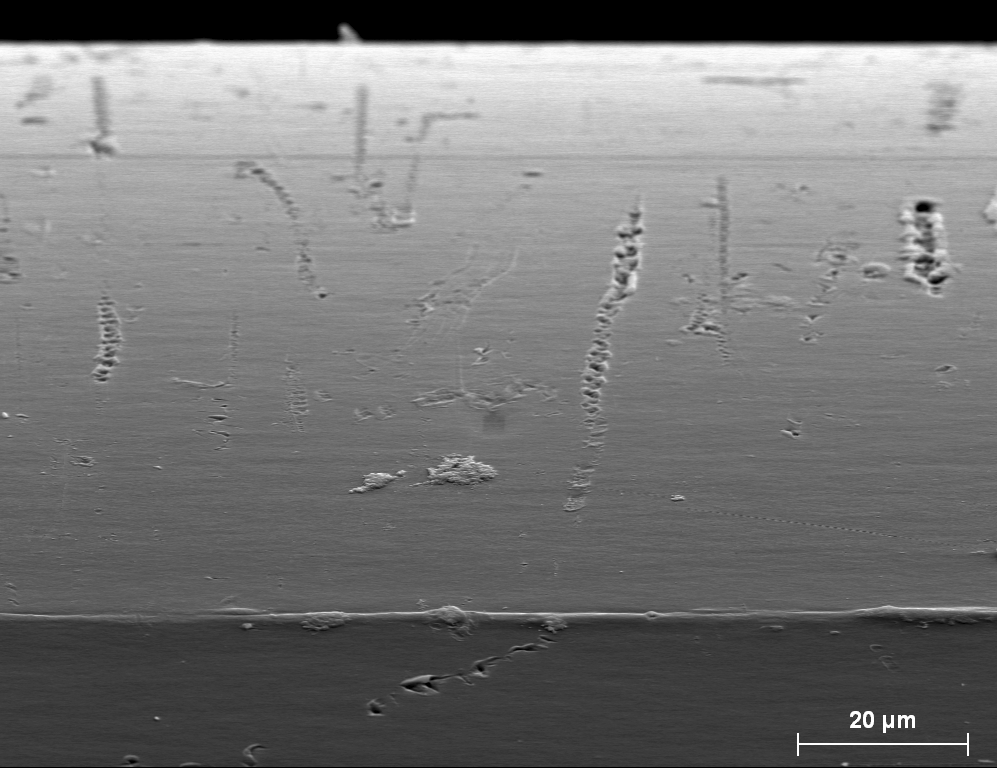
\includegraphics[width=70mm]{./Figuras/sinclad_6_SE.png}}
\caption{Suface of scintillating fibers under electron microscope.} \label{fig:FiberSurfaceElectronMicroscope}
\end{figure}

It has a lot of irregularities and, due to that, we had a loss of light, overall, in the curve of the fibers. It was checked with a simply set-up which is shown in the figure \ref{fig:CurveLight}.

\begin{figure}[htb]
\centering
{
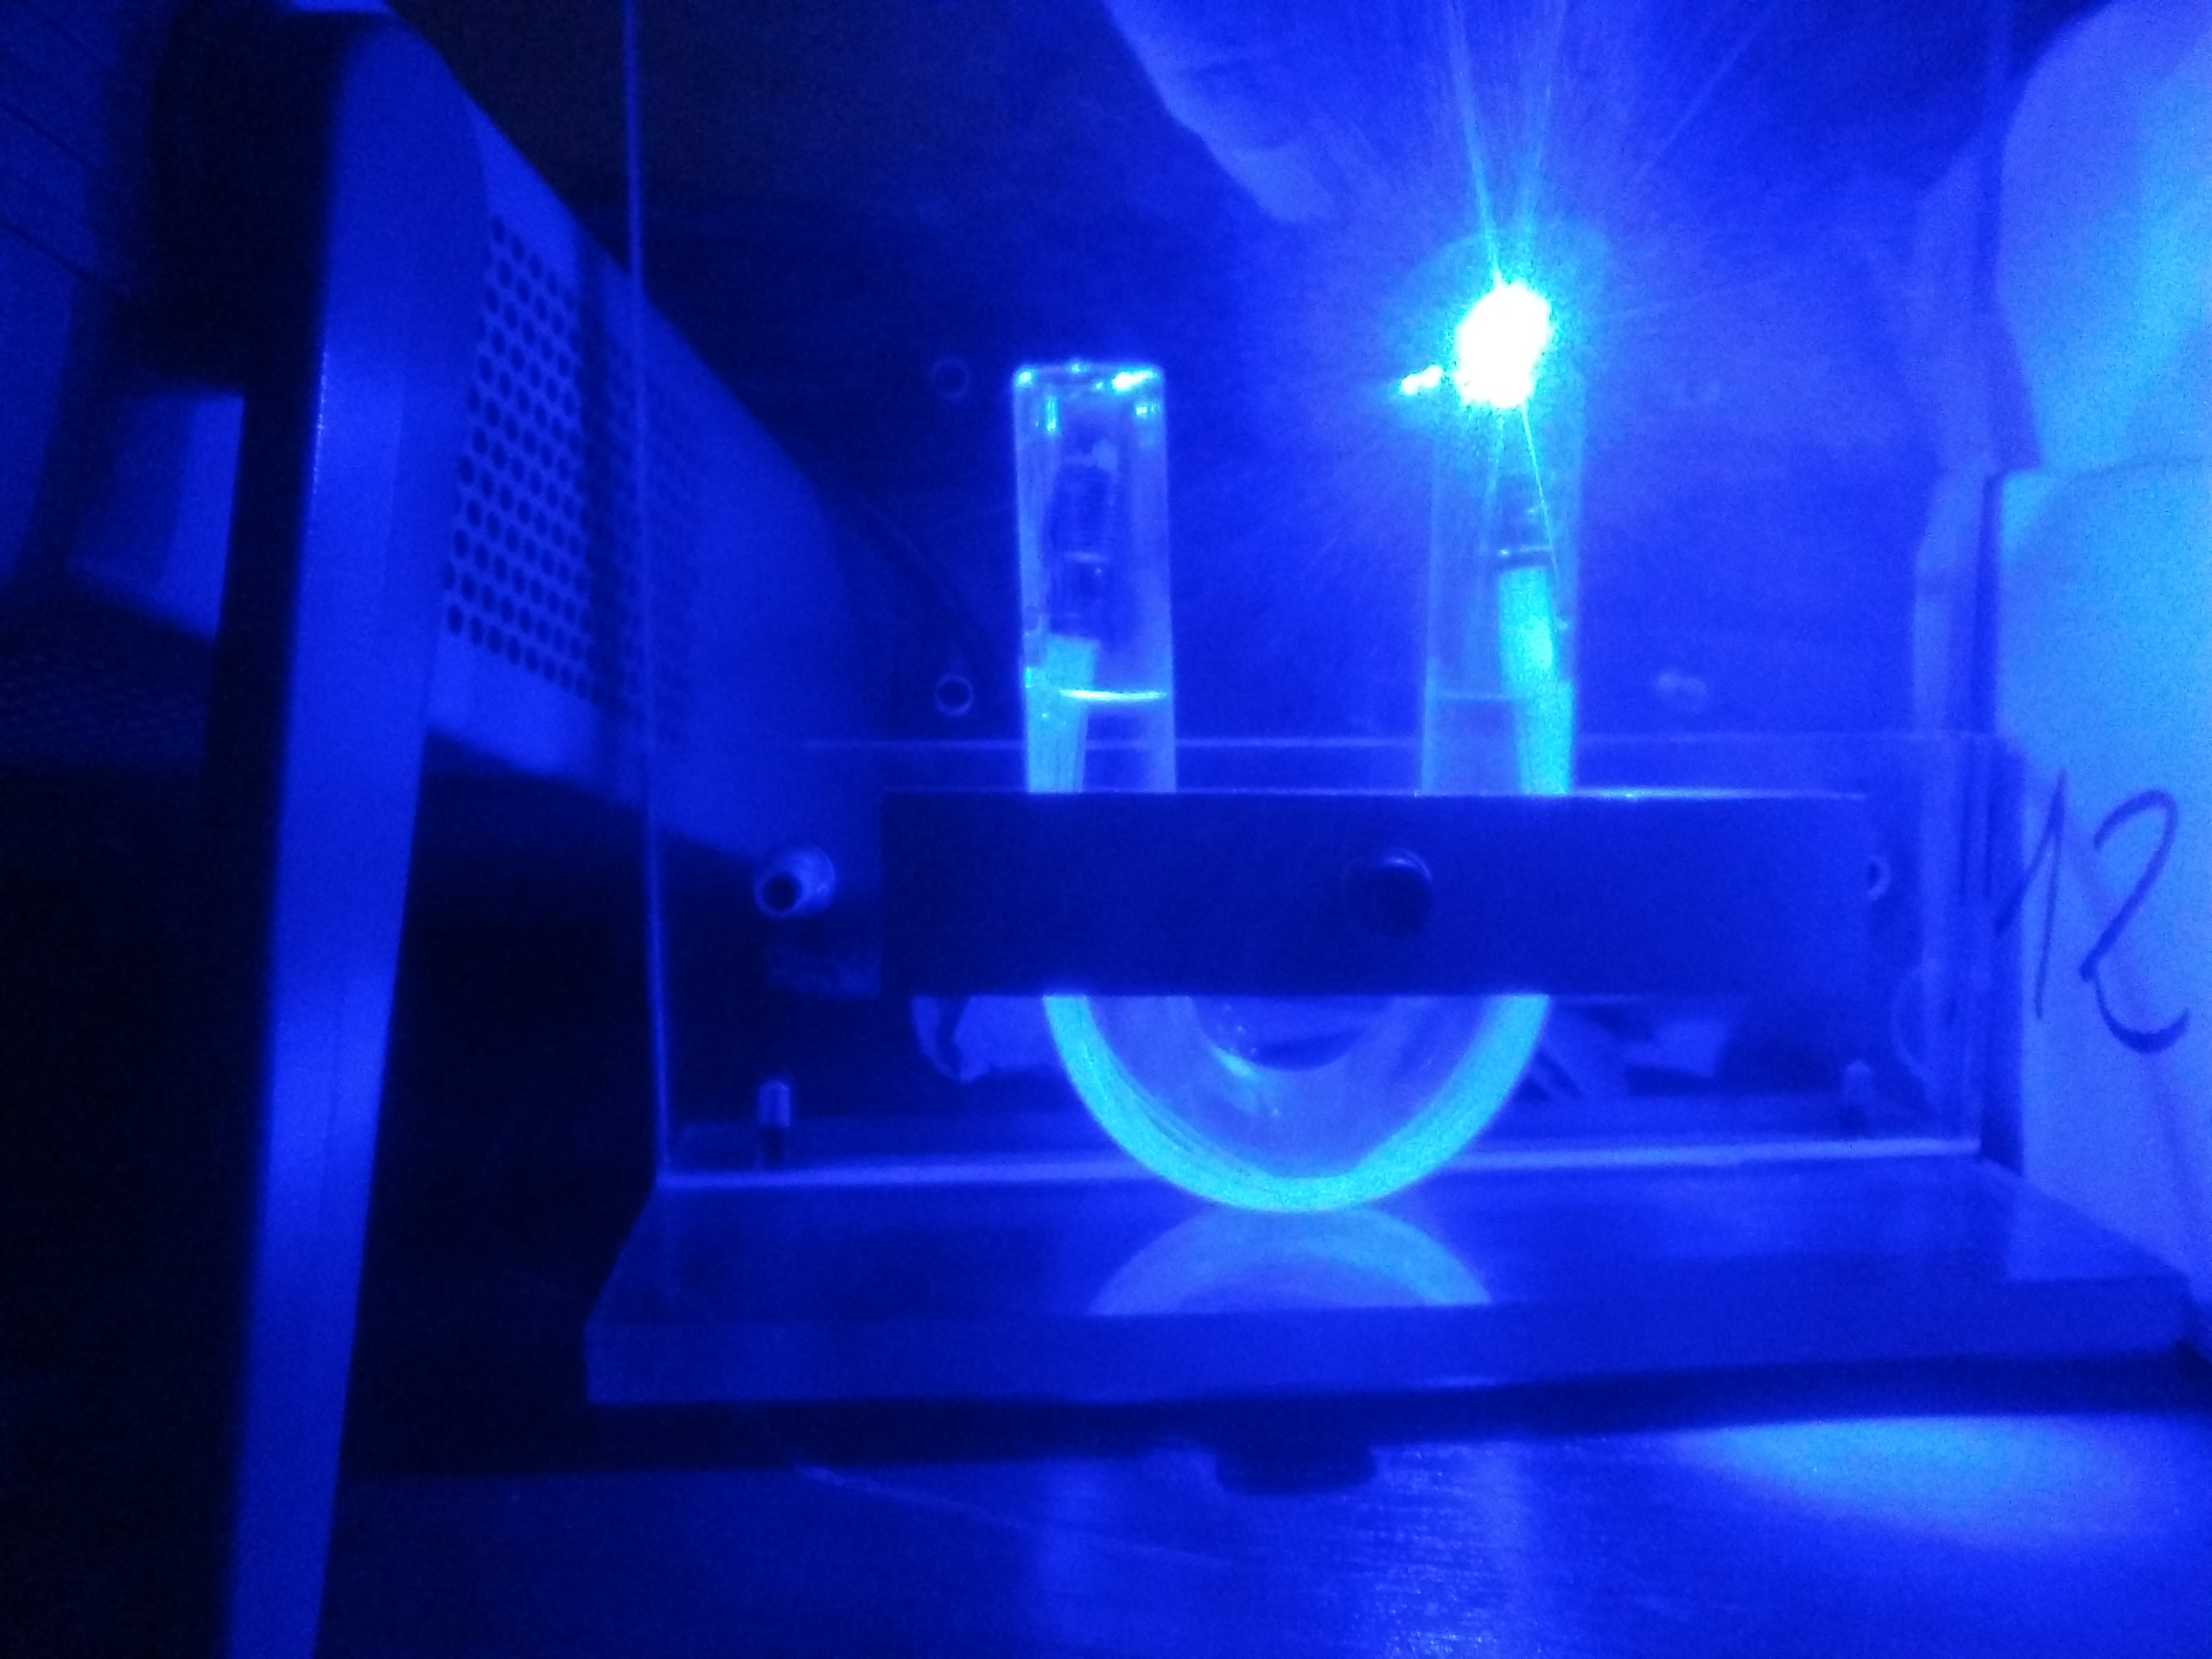
\includegraphics[scale=0.12]{CurveLight.jpg} 
}
\caption{Loss of light due to the curve of the fibers. \label{fig:CurveLight}}
\end{figure}

As a result of this photons losing, we loss some events and, by extension, the efficiency of our detector will be smaller.

Another possible reason for this low efficiency is due to the strong bonding of the fibers. As you can see in the figure \ref{fig:Metalic_piece_bunch}, there are two metalic pieces in each fiber bunch, which join the fibers strongly and, due to that, the water cannot cross among these fibers. It produces that the active area of our detector is smaller and, thus, the specific efficiency of our detector are higher.

\begin{figure}[htbp]
\centering
{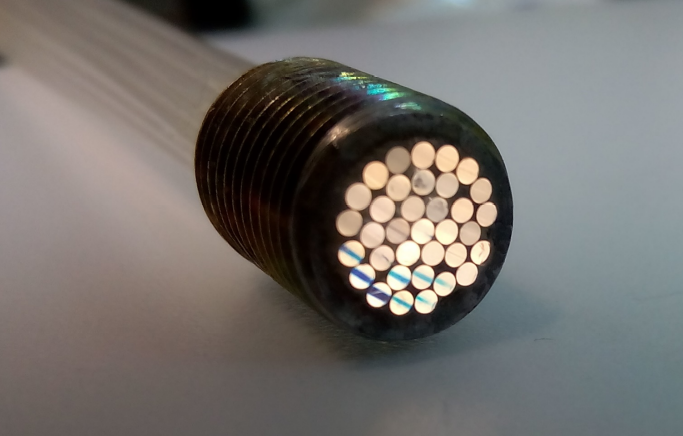
\includegraphics[width=70mm]{./Figuras/Metalic_piece_bunch_fibers.png}}\hspace{10mm}
{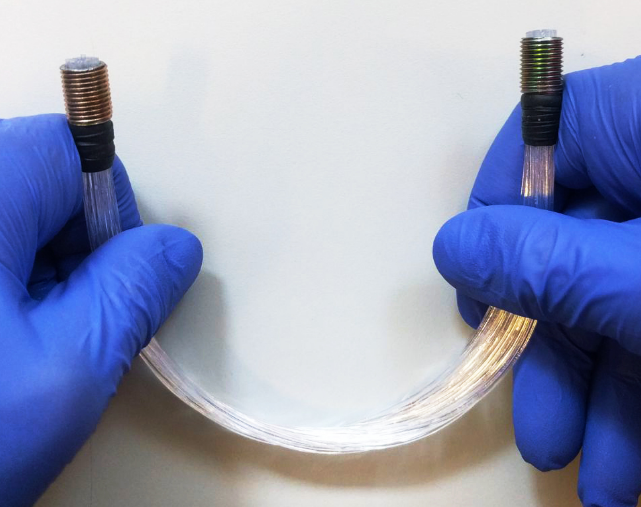
\includegraphics[width=70mm]{./Figuras/bunch_fibers.png}}
\caption{Metal pieces used in the fiber bunch of Tritium-IFIC 0 prototype} \label{fig:Metalic_piece_bunch}
\end{figure}


%\newpage
\section{Tritium-IFIC 1 prototype} \label{sec:TritiumIFIC1}
The name of the second prototype, which has been developed in Valencia, is Tritium-IFIC 1 that is shown in the figure \ref{fig:Tritium_IFIC_1}. This prototype has a internal volume of $0.118~\liter$ and 64 scintillating fibers read out by the same PMT that in the previous prototype. 

In this prototype, the problems found in the first prototype was solved. As we cannot change the quality of the fiber surface we will try to mitigate their effect.

\begin{figure}[htbp]
\centering
\subfigure[Protoype of Tritium-IFIC 1\label{fig:TritiumIFIC1prototype}]
{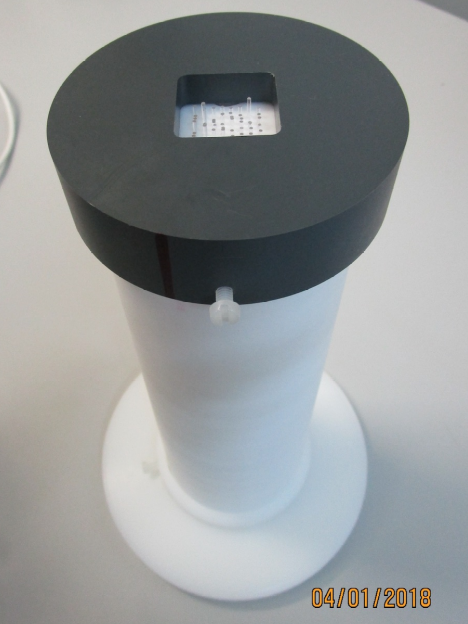
\includegraphics[width=40mm]{./Figuras/Prototype_Tritium_1.png}}\hspace{10mm}
\subfigure[Hole matrix \label{fig:FiberArrangement1}]
{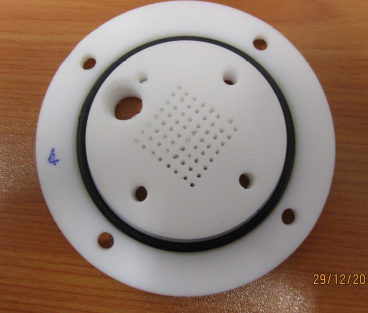
\includegraphics[width=50mm]{./Figuras/Arrange_fibers_piece.png}}\hspace{10mm}
\subfigure[Fiber arrangement matrix \label{fig:FiberArrangement2}]
{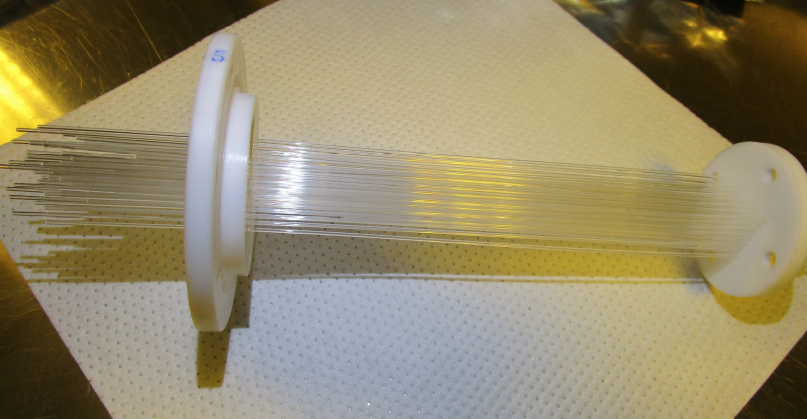
\includegraphics[width=100mm]{./Figuras/Arrange_fibers.png}}
\caption{Tritium-IFIC 1 prototype.} \label{fig:Tritium_IFIC_1}
\end{figure}

First, as you can see in the figure \ref{fig:FiberArrangement2}, the fibers of this detector will be arranged straight, that is, without any curve. With this change we got minimize the amount of photons which escape from the fibers.

Second, we arrange the fibers in a equidistant distance between them. We achieved it with several internal hole matrix as you can see in the figure \ref{fig:FiberArrangement1}. The final aspect of this arranged is shown in the figure \ref{fig:FiberArrangement2}. With this structure we ensure that the active volume of our detector is the one which we know and, with it, we can obtain our correct specific efficiency.

On top of that, we have done some modifications with which we hope to improve the efficiency of our detector.

On the one hand, a special fiber cleaning process has been included consisting of several baths with a neutral soap, pure water and isopropanol inside an ultrasound machine, all this process inside a clean room. With this process we get better wetting properties for fibers and, by extension, we will increase the capacity of this prototype for the detection of tritium.

This process were checked in order to be sure that it don't affect to the light production and collection of the fibers, whose result is shown in the figure \ref{fig:CleaningProcess}.

\begin{figure}[htbp]
\centering
\subfigure[Measurement of the light produced in a bunch of $25$ fibers of $20~\cm$ due to the \ce{^{90}Sr} source \label{fig:SrCleaning}]{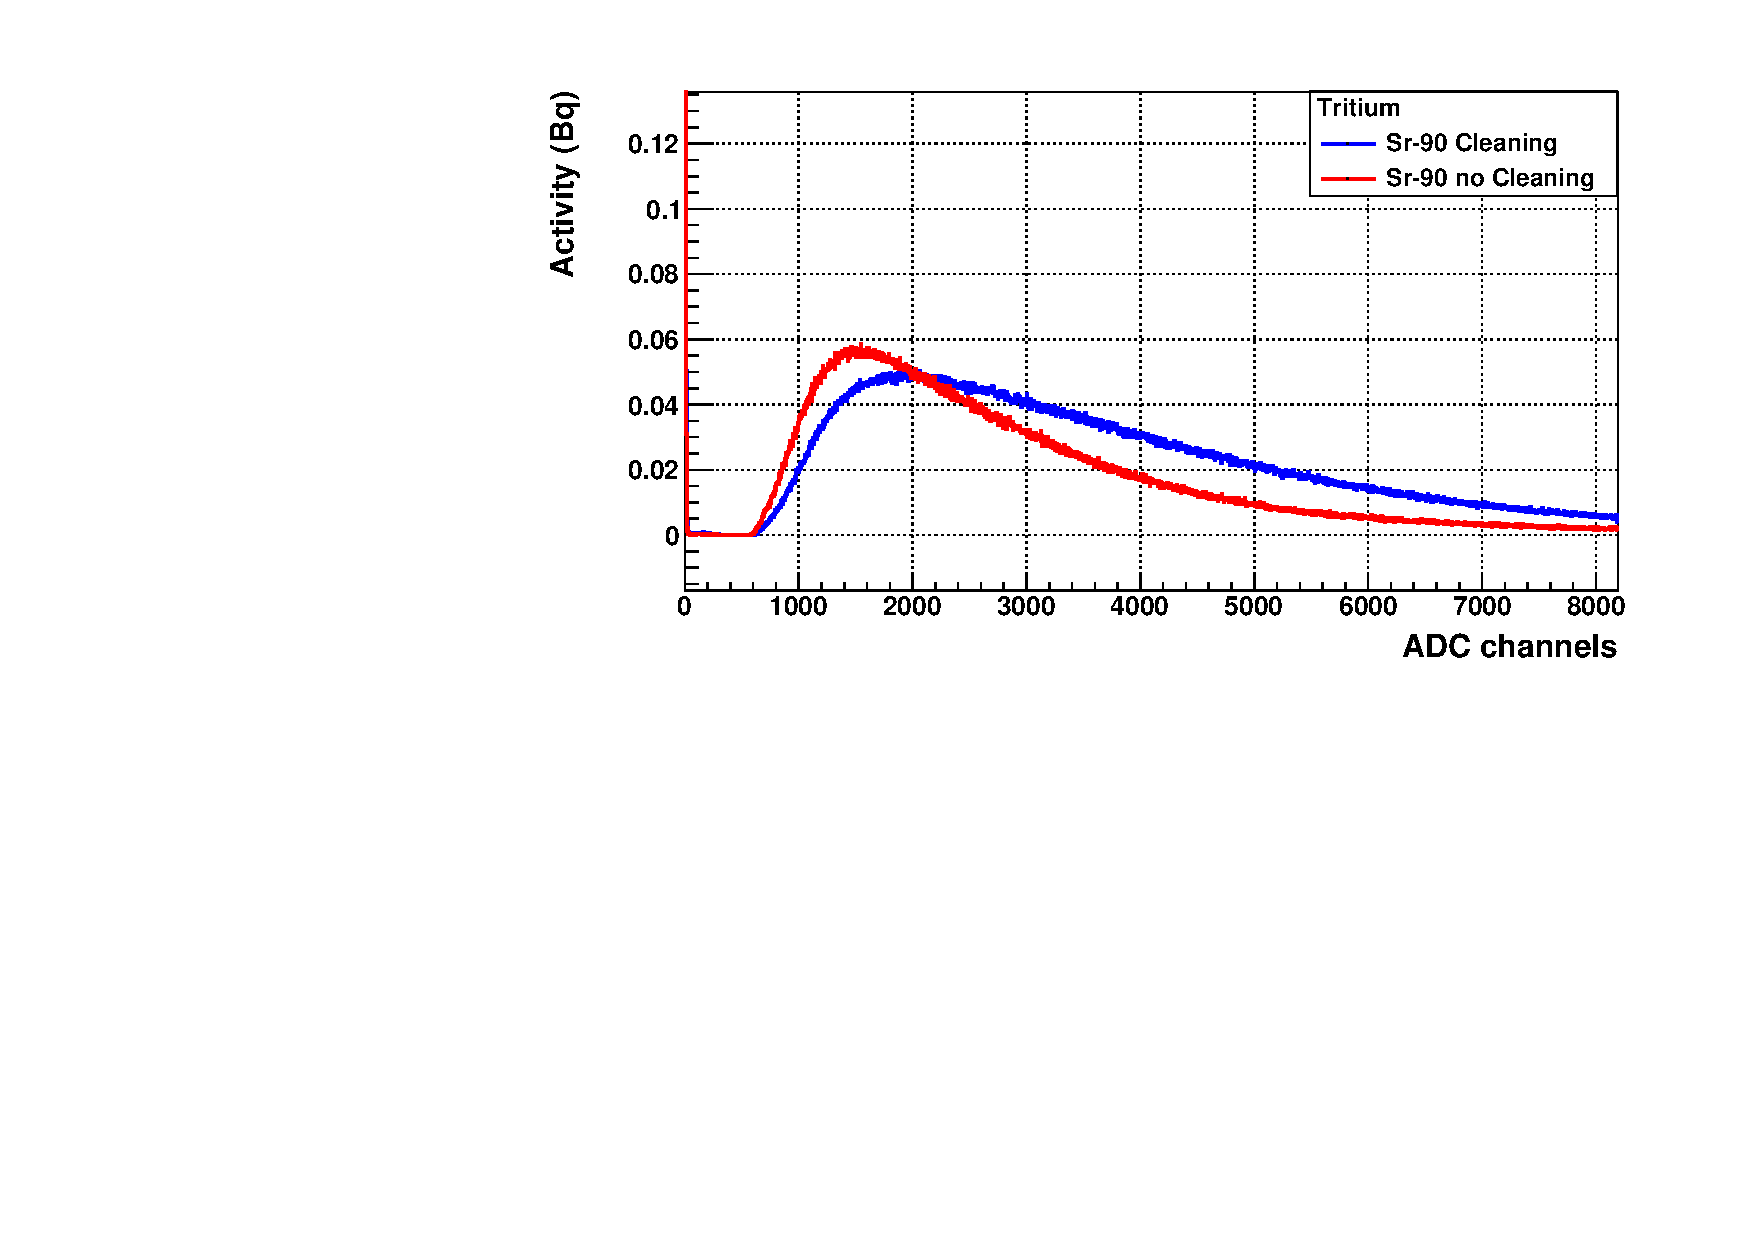
\includegraphics[width=72mm]{./Figuras/Sr_90s.pdf}}\hspace{10mm}
\subfigure[Measurement of the light produced in a bunch of $25$ fibers of $20~\cm$ due to the \ce{^{137}Cs} source \label{fig:CoCleaning}]{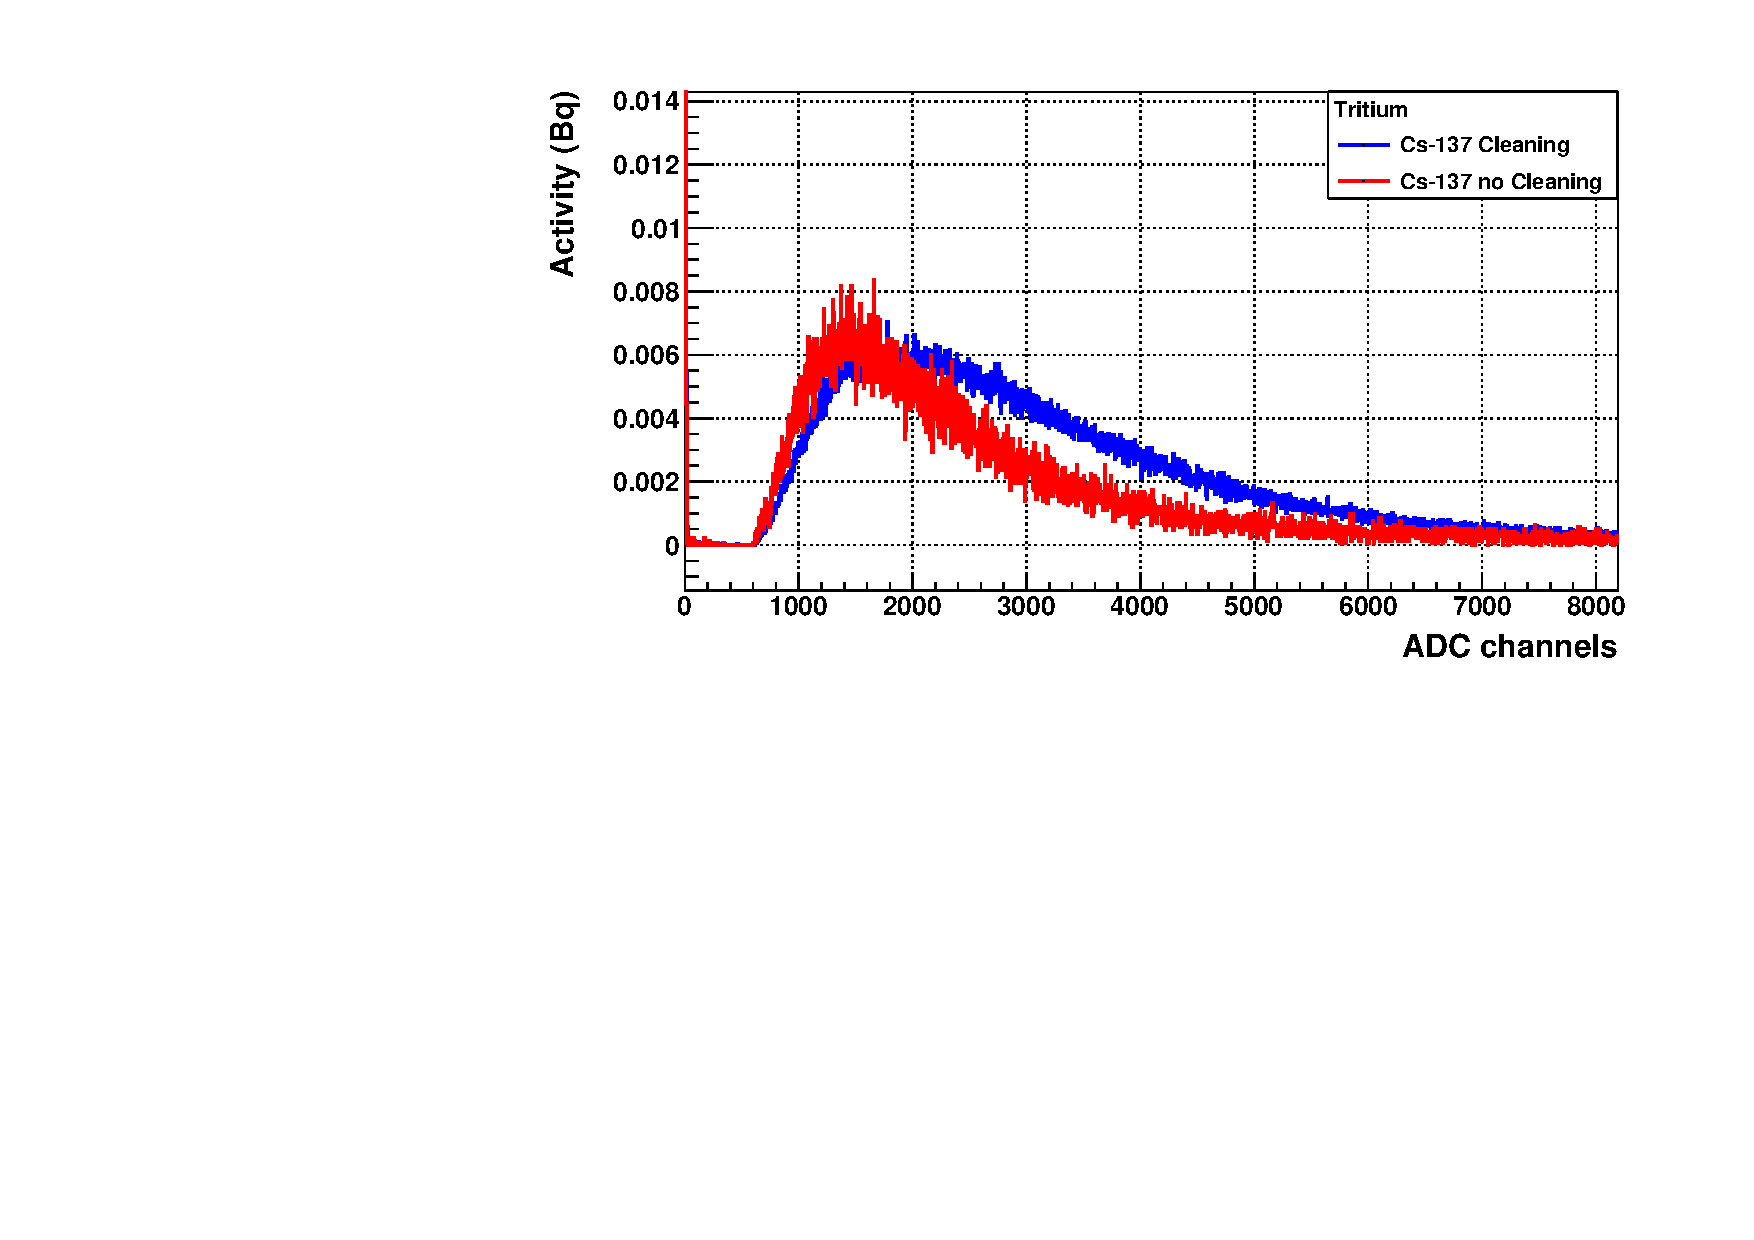
\includegraphics[width=72mm]{./Figuras/Cs_137s.pdf}}
\caption{Cuantification of the improvement of polishing process} \label{fig:CleaningProcess}
\end{figure}

Here we can see that not only it doesn't get worse the light collection efficiency of the fibers but this process improve it. We can see that in both cases event numbers is quite similar but this events has higher energy.

On the other hand we have used teflon for the material of the vessel since its reflectivity is quite similar to 100\%. Therefore if any  photon escape from the fiber it can arrive to any wall of the vessel and come back to the fiber. It will increse the efficiency of our detector.

After we do all this modifications we did the same measurements for check the efficiency of this detector, that's is, one for getting the background signal of our system and another for the tritium signal whose activity was the same that the experience with the previous prototype, $53.385~\mega\becquerel/\liter$. 

We have to take into account that with this prototype we don't make coincidence because this prototype only can measure by one side of the fibers. It is not important because we still use the discriminator with which we remove the termical noise of the PMTs. Other events which we don't remove with this discriminator, like cosmic events with higher energy, it affect statistically equal to the background than the signal, thus, it don't affect to the tritium signal (difference)

The measurements which was done with  this prototype is shown in the figure \ref{fig:Tritium_IFIC_1_Signals}.

\begin{figure}[htbp]
\centering
\subfigure[Signal and Background of Tritium-IFIC 1 \label{fig:SignalsTritiumIFIC1}]{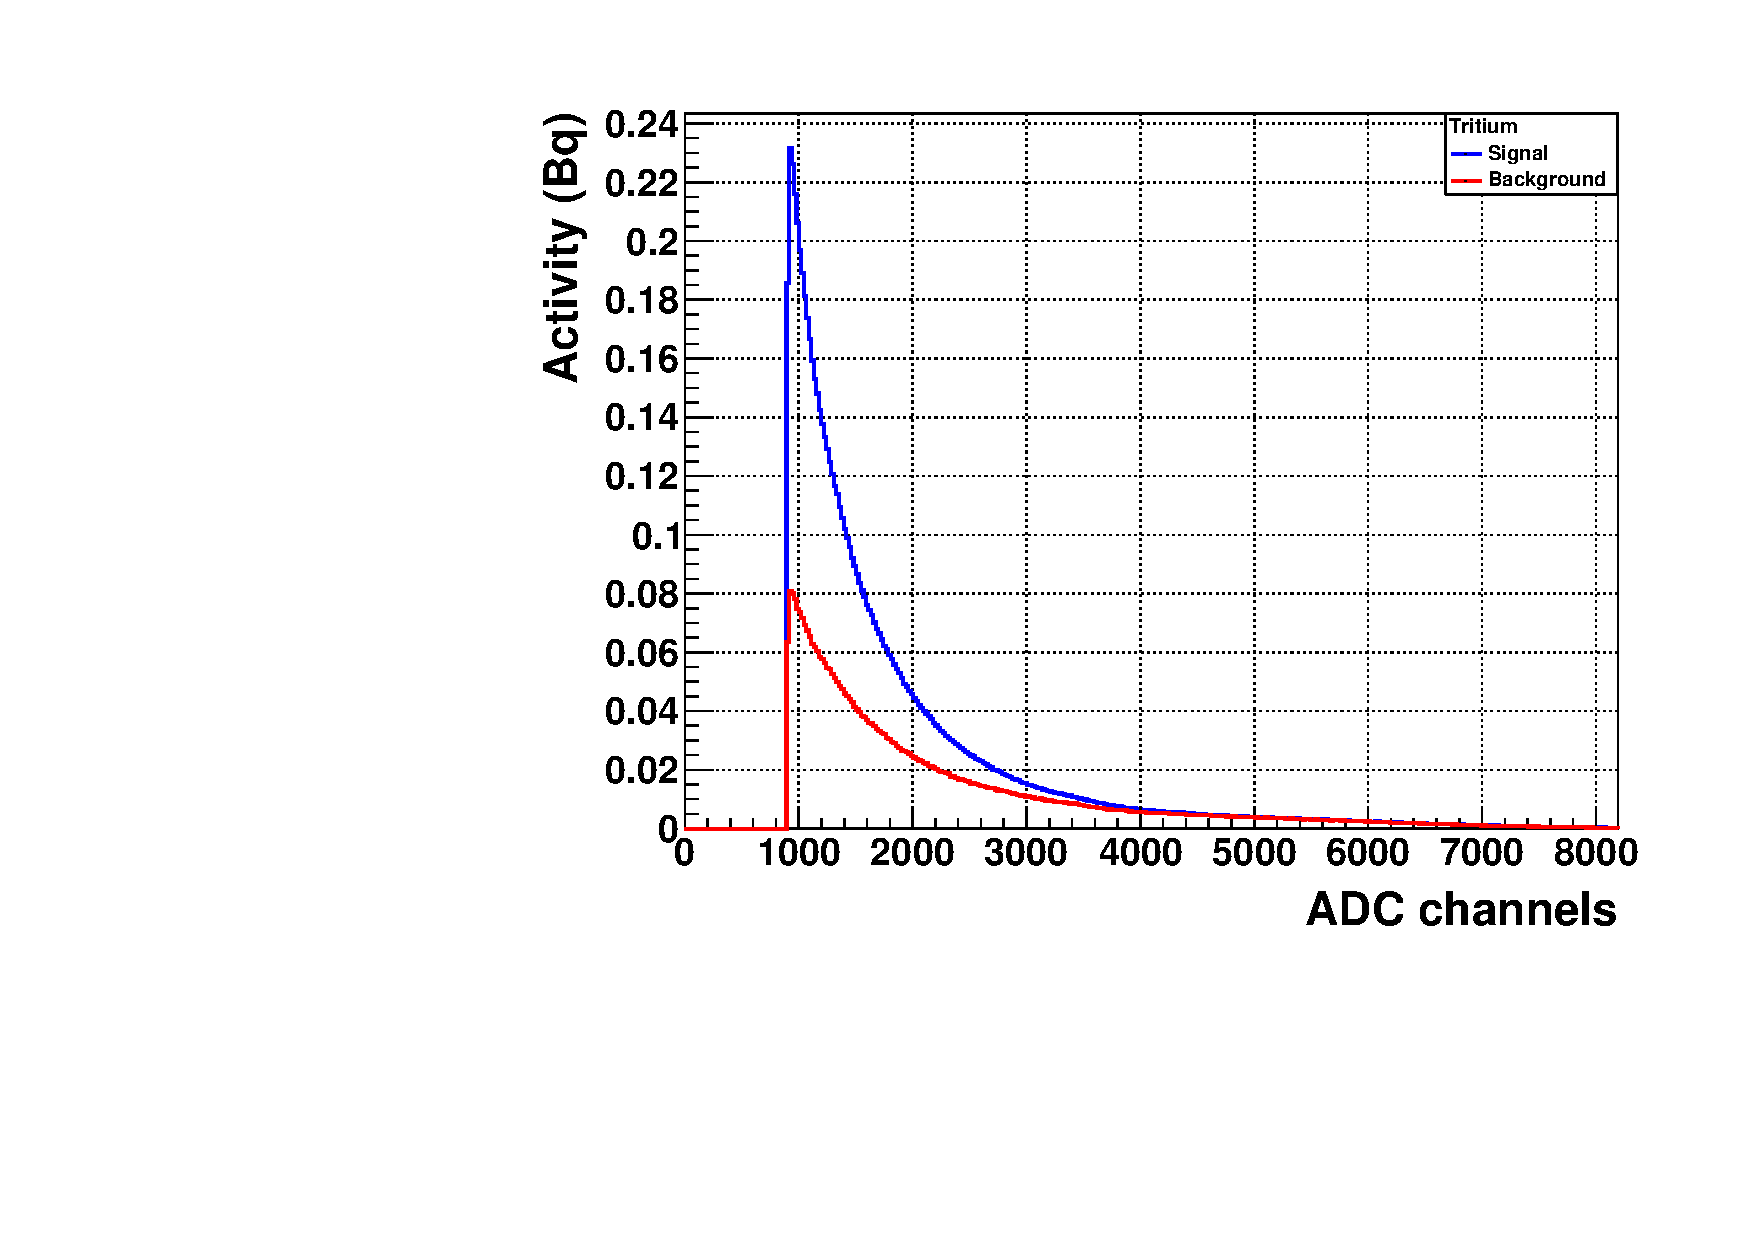
\includegraphics[width=70mm]{./Figuras/Signal_Background_Tritium1.pdf}}
\subfigure[Clear signal of tritium \label{fig:ClearSignalTritiumIFIC1}]{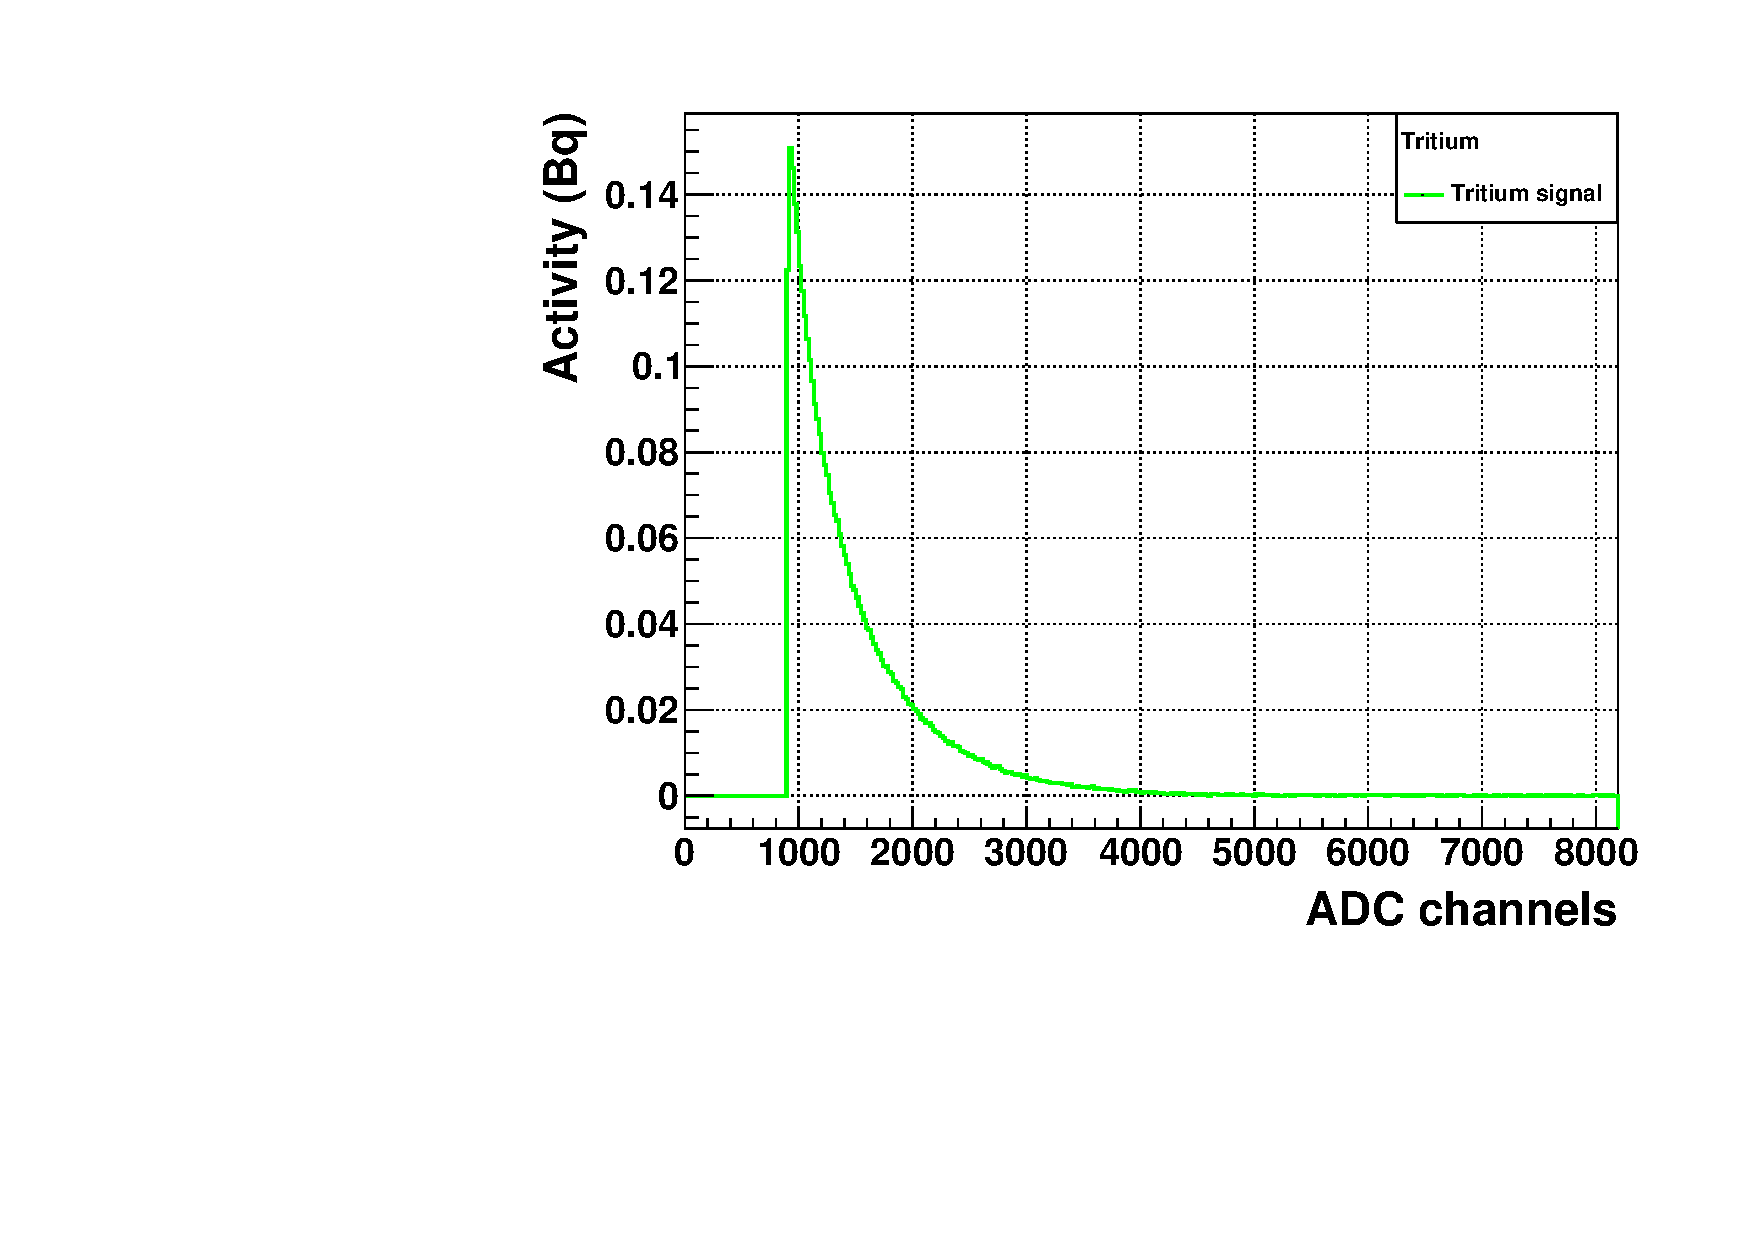
\includegraphics[width=70mm]{./Figuras/Signal_Tritium_Tritium1.pdf}}
\caption{Tritium signals of Tritium-IFIC 1 prototype.} \label{fig:Tritium_IFIC_1_Signals}
\end{figure}

We have obtained $4.17$ counts per second with this prototype and this tritium solution. It means that the efficiency of this prototype is $\varepsilon_{det} = 7.81 \cdot 10^{-5}~(\ce{counts}/\sec)/(\kilo\becquerel/\liter)$. Now the active surface is $A_{suf} = 402.124~\cm^2$ so the specific efficiency is $\varepsilon_{spe} = 1.94 \cdot 10^{-7}~(\ce{counts}/\sec)/(\cm^{2}\kilo\becquerel/\liter)$. 

We can see that our efficiency has improved in a ten factor. In any case it is one order smaller that the efficiency of other detectors with the same objective. It could be due to the pile-up of our system since we are working with higher tritium activities than the other experiments. We are working with activities of the order of $10^{7}~\becquerel/\liter$  and the other experiments was done with activities of the order of $10^{4}~\becquerel/\liter$. It could affect to our measurements in several ways like pile-up or producing a damage of the fibers, both effects contribute to reduce the efficiency of this prototype. It is something which we will check in a near future with prototypes fill with lesser activities of the tritium solution.

The only problem which we have found with this prototype is that we cannot read with two PMTs in coincidence. It is a problem because, although most of the PMT dark current does not overcome the discriminator level, we have to take into account that this discriminator level is very low  since the energy events of tritium are very small. Due to that, it is possible, but unlikely, that some dark current events of the PMT overcome it and contribuite to the signal of the detector. 

%\newpage
\section{Tritium-IFIC 2 prototype} \label{sec:TritiumIFIC2}
The name of the last prototype, which has been developed in Valencia in the framework of tritium project, is Tritium-IFIC 2. In this prototype, which is showed in the figure \ref{fig:Tritium_IFIC_2}, we have increased the number of fibers used up to 800 which are read out by the same PMTs that we used in the previous experiences. Furthermore, these fibers won't be fixed to a hole matrix like Tritium-IFIC 1 because it is difficult with 800 fibers. In this prototype fibers will be free with they have enough freedom in order to allow the flow of the water through them. 

With this prototype we try to solve the problem that we had with Tritium-IFIC 1 related to the coincidence. 

This prototype is expected to be the last one from which we will build our final detector so, although the water won't flow through this laboratory prototype, it has some modifications in order to be prepared with requirements enough to do so. For example, the internal volume will be circular instead of square like the previous prototype as yo can see in the figure \ref{fig:Tritium_IFIC_2_b}. The reason of that is because, although we would like to keep the internal volume square because the active area of the photosensors is square, a circular internal volume is necessary to facilitate the flow of water. The diameter of this circular volume will be enough large to adjust the square active area of the photosensors inside. Due to that, we will have some scintillating fibers which we don't read, at least directly, but it won't be a problem because it is a cheap material. We will only read, at least directly, more than 500 out of 800 fibers.

\begin{figure}[htbp]
\centering
\subfigure[\label{fig:Tritium_IFIC_2_a}]{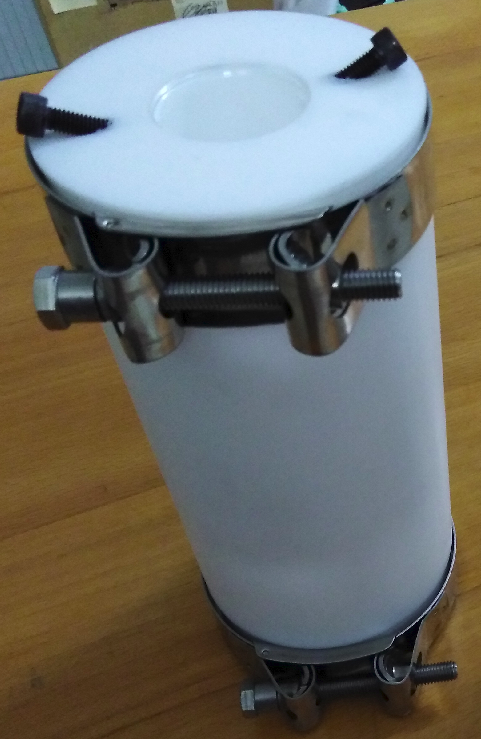
\includegraphics[width=70mm]{./Figuras/Tritium_IFIC_2.png}}
\subfigure[\label{fig:Tritium_IFIC_2_b}]{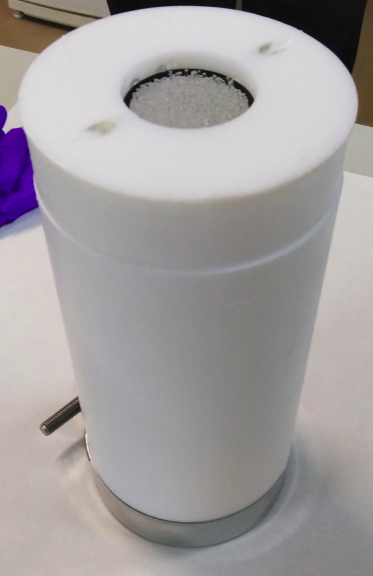
\includegraphics[width=70mm]{./Figuras/Tritium_IFIC_2_2.png}}
\caption{Tritium-IFIC 2 prototype} \label{fig:Tritium_IFIC_2}
\end{figure}

In our last prototypes we have read the fibers directly because in all cases it was on top of the detector. However, it is impossible with this prototype because, as we have seen in our last experiences, we need to keep the fibers straight and read them from both sides so we cannot put both fiber sides on the top of the detector. If the fibers is read on directly, the tritium solution could leak from the side of the fiber that is not on top. 

Therefore, in this prototype, we need a totally closed container inside of which we have the fibers and the tritium solution, whose internal volume is $0.082~\liter$. This container is filled from two holes at the top of the prototype and it has two windows to read the fibers, as you can see in figure \ref{fig:Tritium_IFIC_2}, one at the top of the prototype and one at the bottom. The material of these windows will be PMMA (polymethyl methacrylate) because the light transmission in this material is close to $100\%$ so we don't loss photons and, by extensions, it don't affect to the efficiency of our detector.

Finally a aluminium structure was built for hold several prototypes like it. This structure is shown in the figure \ref{fig:Tritium_IFIC_2_holder}.

\begin{figure}[htbp]
\centering
\subfigure[\label{fig:Tritium_IFIC_2_holder_a}]{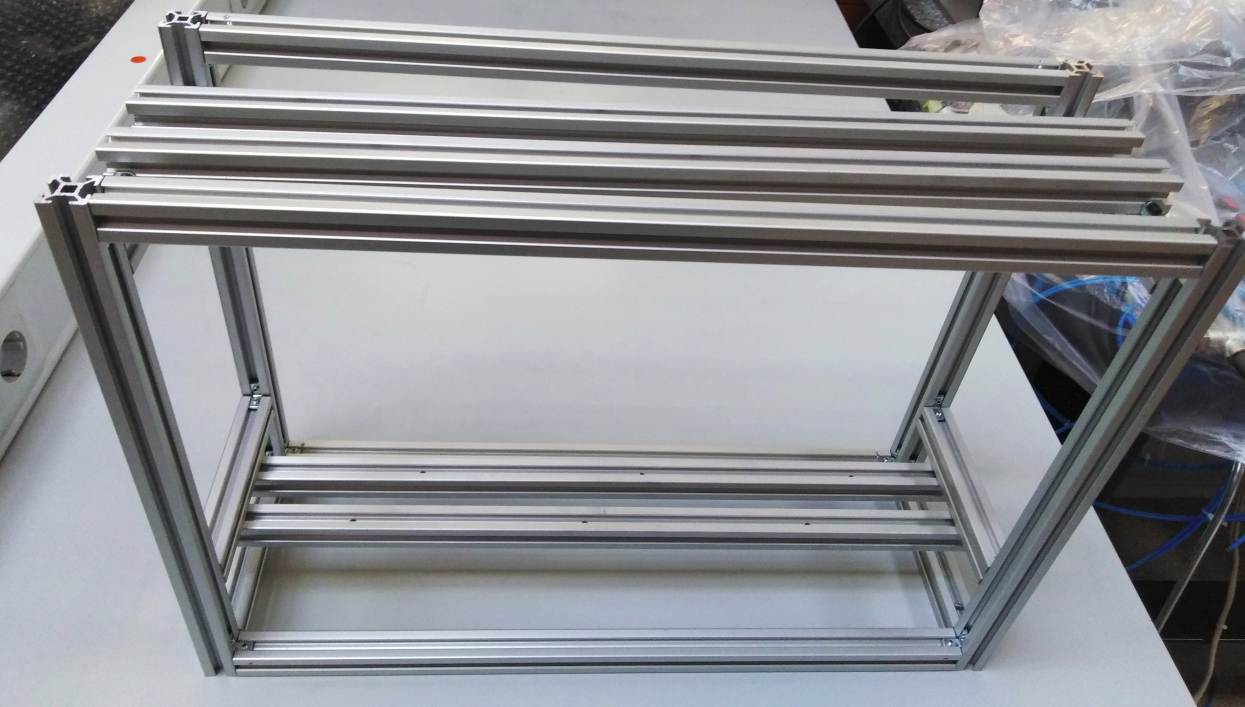
\includegraphics[width=70mm]{./Figuras/Tritium_IFIC_2_Holder.png}}
\subfigure[\label{fig:Tritium_IFIC_2_holder_b}]{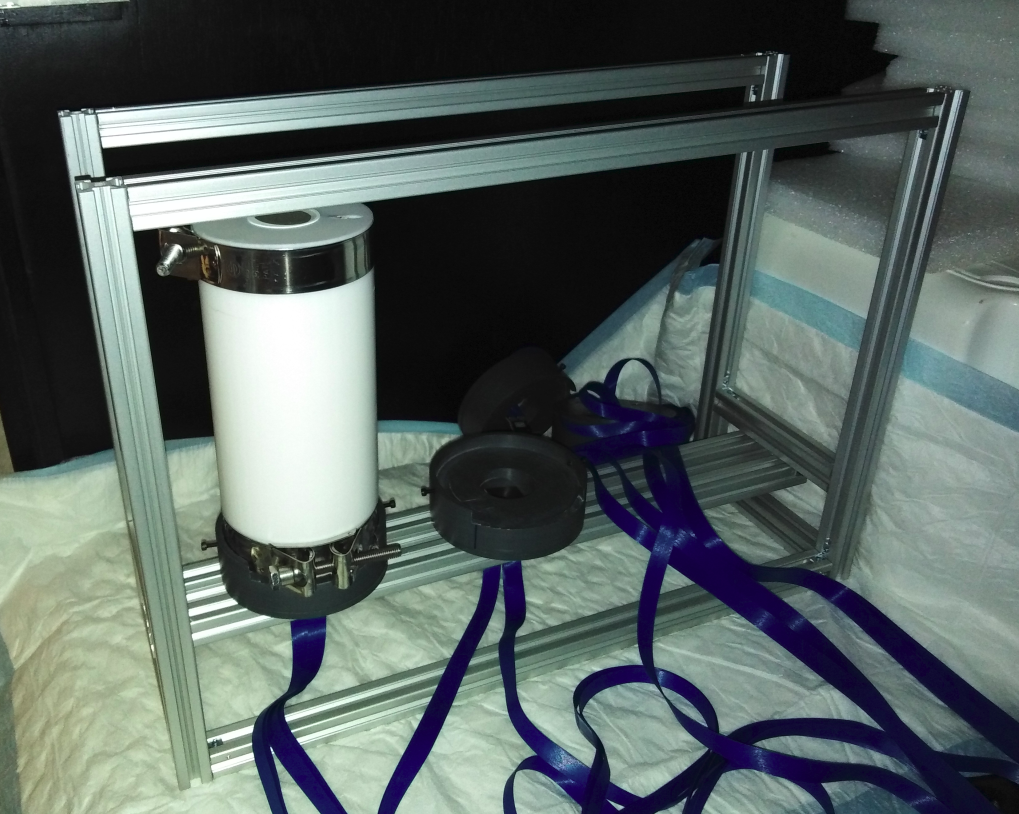
\includegraphics[width=70mm]{./Figuras/Tritium_IFIC_2_Holder_2.png}}
\caption{Tritium-IFIC 2 prototype} \label{fig:Tritium_IFIC_2_holder}
\end{figure}

Similarly like past experiences, the measurements obtained for the background signal and the tritium signal with the same tritium activity are shown in the figure \ref{}:

FIGURAS

CALCULO DE EFICIENCIAS.

In order to check the difference between PMTs and SiPM arrays we repite this experiences but using SiPM arrays as a photosensors. The SiPM arrays used in these experiences are commercial from Hamamatsu, whose serial number is S13361-6075AE-04. It has higher photodetection efficiency, $50\%$ than PMTs, less than $30\%$, so they should get better results. The measurements obtained in this experience is shown in the figure \ref{}

FIGURAS

CALCULA DE EFICIENCIAS

DISCUSIÓN DE CUAL ES MEJOR.


%\newpage
\section{Conclusions} \label{sec:Conclusions}
Three different prototypes has been developed in the framework of the tritium project for detection of tritium activities in the water which is used by Nuclear Power Plants. In each detector several improvements has been included in order to increase their efficiency and reduce the LDL (Low Detection Level) of tritium. 

The table \ref{} summarize the most important parameters of each prototypes.

TABLE

CONCLUSIONS

The next step will be to install in arrocampo nuclear power plant three detectors like Tritium-IFIC 2, which we will call cells. 

The cells are essentially the same as the prototype. These have minimal differences which are necessary to work in Arrocampo since the water needs to flow through the cells. In the picture \ref{fig:Cell_prototype} we can see both, a Tritium-IFIC 2  prototype and one cell. 

\begin{figure}[htb]
\centering
{
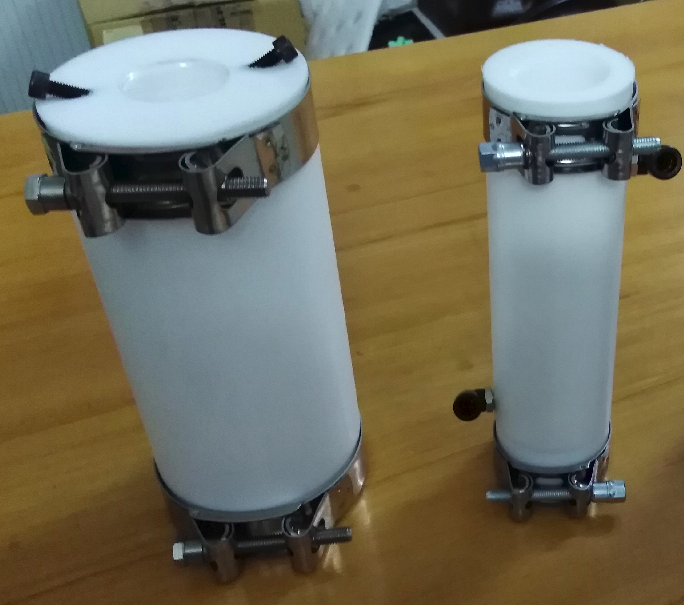
\includegraphics[scale=0.25]{Cell_Tritium_IFIC_2.png} 
}
\caption{Tritium-IFIC 2 prototype in the left size and Cell of Tritium detector in the right side \label{fig:Cell_prototype}}
\end{figure} 


There we can see that the cells are thinner than the Tritium-IFIC 2 prototype. This is because we don't need the holes in the top of the detector, whose function is to fill the prototype. Instead of that, water will flow continuously through the cells so we need two pieces in the cells (black pieces) from where the water will enter to the cell, it will cross the fibers and it will leave the cell. All these differences are little modifications which souldn't affect the the detector efficiency.

First we will install three identical cells that we will read in parallel. With this parallel reading we won't improve its efficiency, it will only be maintained, but we will reduce their LDL which is very important because the activity which we want to detect follow the ALARA principle (As Low As Possible Achievable). If it is necessary we can install more cells that we can read in parallel, as many as we need for arriving to our objective, $100~\becquerel/\liter$

%\newpage
\section{Appendice A: Protocol following for filling in the tritium prototypes} \label{sec:FillInPrototypes}
\input{./Secciones/9FillInPrototypes}
\end{document}